%% =====================================================================
%%  EVERY EXHIBIT IN THE LIVE MANUSCRIPT, RECOMPUTED WITH THE TWO
%%  INCREDIBLE WEIGHT GUESSERS DROPPED
%%
%%  Generated 2026-08-21. Pipeline: all 25 scripts in scripts/python run
%%  with EXCLUDE_INCREDIBLE_GUESSERS=1.
%%
%%  SCOPE
%%  The exhibit list is taken from manuscript/main.log, i.e. what the live
%%  document actually compiles, not from grepping the sources. Commented-out
%%  exhibits and tables belonging to the pre-restructure draft are excluded.
%%  Contents: 5 tables + 7 figures = 12 exhibits, in document order.
%%
%%  EXCLUSION CRITERION
%%  A guess is credible if non-zero. Every non-zero guess in the data lies
%%  between 114 and 253 lbs, a plausible adult body weight throughout.
%%  Credible-guess counts over the ten rounds are 10 for 158 subjects, then
%%  7, then 2, then 0. Any cutoff between 3 and 7 selects the same two.
%%
%%  DROPPED (Player A 161 -> 159; total 322 -> 320)
%%    code d8goj7g9   2 of 10 credible   (0,0,0,0,0,0,0,148,0,174)
%%    code pd4bg6c3   0 of 10 credible   (all ten rounds zero)
%%  Both in session t9ih1lzz. Both are No-Punishment non-delegators, which
%%  is why dropping them widens the H1 gap from 16.8pp to 18.3pp
%%  (chi-square p 0.033 -> 0.021).
%%
%%  KEPT, boundary case
%%    code 7o6vx9ld   7 of 10 credible   (187,213,114,0,171,0,184,137,117,0)
%%
%%  Each exhibit below is tagged [CHANGED] or [IDENTICAL] against the live
%%  version. 5 of 12 change; the 7 punishment-side and belief exhibits do
%%  not, because both dropped subjects are Player A.
%%
%%  THE LIVE MANUSCRIPT IS UNTOUCHED. tables/, manuscript/figures/ and
%%  numbers.json were restored byte-identical after the run.
%%
%%  USAGE
%%    %% =====================================================================
%%  EVERY EXHIBIT IN THE LIVE MANUSCRIPT, RECOMPUTED WITH THE TWO
%%  INCREDIBLE WEIGHT GUESSERS DROPPED
%%
%%  Generated 2026-08-21. Pipeline: all 25 scripts in scripts/python run
%%  with EXCLUDE_INCREDIBLE_GUESSERS=1.
%%
%%  SCOPE
%%  The exhibit list is taken from manuscript/main.log, i.e. what the live
%%  document actually compiles, not from grepping the sources. Commented-out
%%  exhibits and tables belonging to the pre-restructure draft are excluded.
%%  Contents: 5 tables + 7 figures = 12 exhibits, in document order.
%%
%%  EXCLUSION CRITERION
%%  A guess is credible if non-zero. Every non-zero guess in the data lies
%%  between 114 and 253 lbs, a plausible adult body weight throughout.
%%  Credible-guess counts over the ten rounds are 10 for 158 subjects, then
%%  7, then 2, then 0. Any cutoff between 3 and 7 selects the same two.
%%
%%  DROPPED (Player A 161 -> 159; total 322 -> 320)
%%    code d8goj7g9   2 of 10 credible   (0,0,0,0,0,0,0,148,0,174)
%%    code pd4bg6c3   0 of 10 credible   (all ten rounds zero)
%%  Both in session t9ih1lzz. Both are No-Punishment non-delegators, which
%%  is why dropping them widens the H1 gap from 16.8pp to 18.3pp
%%  (chi-square p 0.033 -> 0.021).
%%
%%  KEPT, boundary case
%%    code 7o6vx9ld   7 of 10 credible   (187,213,114,0,171,0,184,137,117,0)
%%
%%  Each exhibit below is tagged [CHANGED] or [IDENTICAL] against the live
%%  version. 5 of 12 change; the 7 punishment-side and belief exhibits do
%%  not, because both dropped subjects are Player A.
%%
%%  THE LIVE MANUSCRIPT IS UNTOUCHED. tables/, manuscript/figures/ and
%%  numbers.json were restored byte-identical after the run.
%%
%%  USAGE
%%    %% =====================================================================
%%  EVERY EXHIBIT IN THE LIVE MANUSCRIPT, RECOMPUTED WITH THE TWO
%%  INCREDIBLE WEIGHT GUESSERS DROPPED
%%
%%  Generated 2026-08-21. Pipeline: all 25 scripts in scripts/python run
%%  with EXCLUDE_INCREDIBLE_GUESSERS=1.
%%
%%  SCOPE
%%  The exhibit list is taken from manuscript/main.log, i.e. what the live
%%  document actually compiles, not from grepping the sources. Commented-out
%%  exhibits and tables belonging to the pre-restructure draft are excluded.
%%  Contents: 5 tables + 7 figures = 12 exhibits, in document order.
%%
%%  EXCLUSION CRITERION
%%  A guess is credible if non-zero. Every non-zero guess in the data lies
%%  between 114 and 253 lbs, a plausible adult body weight throughout.
%%  Credible-guess counts over the ten rounds are 10 for 158 subjects, then
%%  7, then 2, then 0. Any cutoff between 3 and 7 selects the same two.
%%
%%  DROPPED (Player A 161 -> 159; total 322 -> 320)
%%    code d8goj7g9   2 of 10 credible   (0,0,0,0,0,0,0,148,0,174)
%%    code pd4bg6c3   0 of 10 credible   (all ten rounds zero)
%%  Both in session t9ih1lzz. Both are No-Punishment non-delegators, which
%%  is why dropping them widens the H1 gap from 16.8pp to 18.3pp
%%  (chi-square p 0.033 -> 0.021).
%%
%%  KEPT, boundary case
%%    code 7o6vx9ld   7 of 10 credible   (187,213,114,0,171,0,184,137,117,0)
%%
%%  Each exhibit below is tagged [CHANGED] or [IDENTICAL] against the live
%%  version. 5 of 12 change; the 7 punishment-side and belief exhibits do
%%  not, because both dropped subjects are Player A.
%%
%%  THE LIVE MANUSCRIPT IS UNTOUCHED. tables/, manuscript/figures/ and
%%  numbers.json were restored byte-identical after the run.
%%
%%  USAGE
%%    %% =====================================================================
%%  EVERY EXHIBIT IN THE LIVE MANUSCRIPT, RECOMPUTED WITH THE TWO
%%  INCREDIBLE WEIGHT GUESSERS DROPPED
%%
%%  Generated 2026-08-21. Pipeline: all 25 scripts in scripts/python run
%%  with EXCLUDE_INCREDIBLE_GUESSERS=1.
%%
%%  SCOPE
%%  The exhibit list is taken from manuscript/main.log, i.e. what the live
%%  document actually compiles, not from grepping the sources. Commented-out
%%  exhibits and tables belonging to the pre-restructure draft are excluded.
%%  Contents: 5 tables + 7 figures = 12 exhibits, in document order.
%%
%%  EXCLUSION CRITERION
%%  A guess is credible if non-zero. Every non-zero guess in the data lies
%%  between 114 and 253 lbs, a plausible adult body weight throughout.
%%  Credible-guess counts over the ten rounds are 10 for 158 subjects, then
%%  7, then 2, then 0. Any cutoff between 3 and 7 selects the same two.
%%
%%  DROPPED (Player A 161 -> 159; total 322 -> 320)
%%    code d8goj7g9   2 of 10 credible   (0,0,0,0,0,0,0,148,0,174)
%%    code pd4bg6c3   0 of 10 credible   (all ten rounds zero)
%%  Both in session t9ih1lzz. Both are No-Punishment non-delegators, which
%%  is why dropping them widens the H1 gap from 16.8pp to 18.3pp
%%  (chi-square p 0.033 -> 0.021).
%%
%%  KEPT, boundary case
%%    code 7o6vx9ld   7 of 10 credible   (187,213,114,0,171,0,184,137,117,0)
%%
%%  Each exhibit below is tagged [CHANGED] or [IDENTICAL] against the live
%%  version. 5 of 12 change; the 7 punishment-side and belief exhibits do
%%  not, because both dropped subjects are Player A.
%%
%%  THE LIVE MANUSCRIPT IS UNTOUCHED. tables/, manuscript/figures/ and
%%  numbers.json were restored byte-identical after the run.
%%
%%  USAGE
%%    \input{../quality_reports/exhibits_excl_incredible_guessers/exhibits_excl_incredible_guessers.tex}
%%  from manuscript/main.tex. Every label carries an excl_ prefix, so this
%%  file can coexist with the live exhibits in a single document.
%% =====================================================================

\clearpage
\section*{Exhibits excluding the two incredible weight guessers}

\clearpage
\subsection*{Results}

%% ---------------------------------------------------
%% delegation_shares  [CHANGED]   live location: results.tex:19
%% ---------------------------------------------------
\begin{figure}[!htbp]
    \centering
    \caption{Delegation shares by condition}
    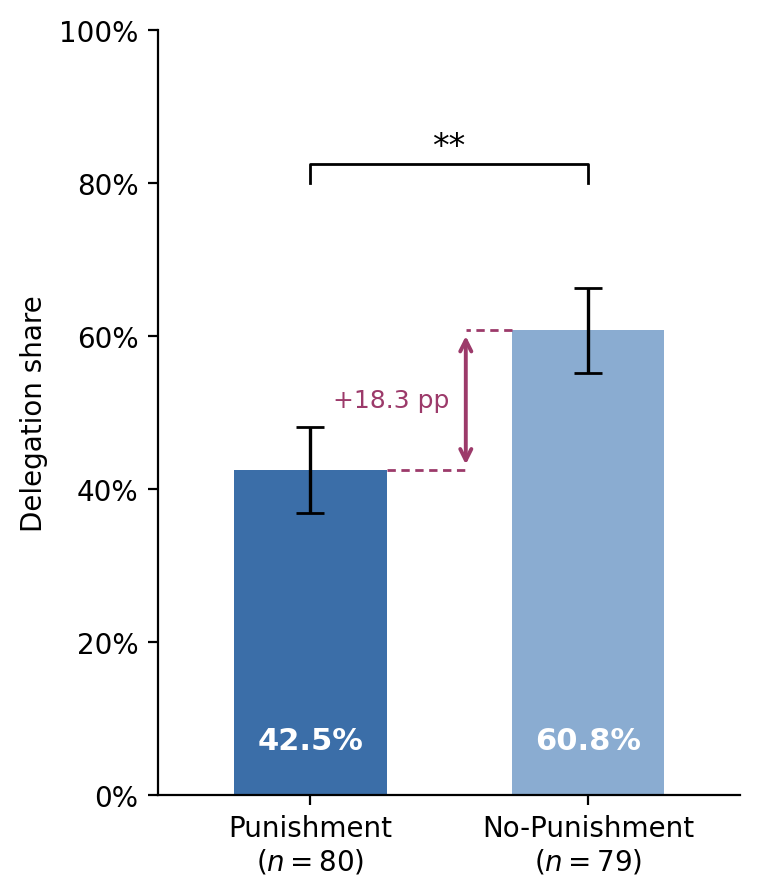
\includegraphics[width=0.5\linewidth]{../quality_reports/exhibits_excl_incredible_guessers/figures/delegation_shares.png}
    \label{fig:excl_delegation_shares}
\end{figure}

\clearpage
%% ---------------------------------------------------
%% reg_delegation  [CHANGED]   live location: results.tex:31
%% ---------------------------------------------------
\begin{table}[!htbp]
\centering
\scriptsize
\caption{Determinants of the delegation decision}
\label{tab:excl_del_decision_determinants}
\begin{tabular}{@{\extracolsep{5pt}}lcccc|c}
\\[-1.8ex]\hline
\hline \\[-1.8ex]
& \multicolumn{5}{c}{Dependent variable: \textit{Delegation}}\\[0.1cm]
& \multicolumn{4}{c}{\textit{Full sample}} & \textit{Passers} \\
\\[-1.8ex] & (1) & (2) & (3) & (4) & (5) \\
\hline \\[-1.8ex]
 Punishment indicator & $-0.462^{**}$ & $-0.473^{**}$ & $-0.537^{**}$ & $-0.489^{**}$ & $-0.589^{**}$ \\
  & $(0.201)$ & $(0.206)$ & $(0.209)$ & $(0.207)$ & $(0.235)$ \\[0.1cm]
 Task performance &  &  & $-0.160^{**}$ &  & $-0.203^{**}$ \\
  &  &  & $(0.081)$ &  & $(0.089)$ \\[0.1cm]
 Perceived performance &  &  &  & $-0.075$ &  \\
  &  &  &  & $(0.057)$ &  \\[0.1cm]
 Age &  & $-0.003$ & $-0.002$ & $-0.002$ & $0.002$ \\
  &  & $(0.009)$ & $(0.009)$ & $(0.009)$ & $(0.011)$ \\[0.1cm]
 Female &  & $0.141$ & $0.194$ & $0.181$ & $0.372$ \\
  &  & $(0.228)$ & $(0.230)$ & $(0.231)$ & $(0.257)$ \\[0.1cm]
 Socio-economic status &  & $-0.044$ & $-0.042$ & $-0.036$ & $-0.086$ \\
  &  & $(0.071)$ & $(0.073)$ & $(0.072)$ & $(0.081)$ \\[0.1cm]
 Went to uni &  & $0.032$ & $0.062$ & $0.020$ & $0.118$ \\
  &  & $(0.228)$ & $(0.226)$ & $(0.227)$ & $(0.248)$ \\[0.1cm]
 Technology score &  & $-0.065$ & $-0.036$ & $-0.056$ & $0.024$ \\
  &  & $(0.093)$ & $(0.096)$ & $(0.093)$ & $(0.109)$ \\[0.1cm]
 Leadership position &  & $0.415^{*}$ & $0.444^{*}$ & $0.411^{*}$ & $0.278$ \\
  &  & $(0.226)$ & $(0.228)$ & $(0.226)$ & $(0.256)$ \\[0.1cm]
 Constant & $0.273^{*}$ & $0.533$ & $0.908$ & $0.801$ & $0.851$ \\
  & $(0.143)$ & $(0.557)$ & $(0.593)$ & $(0.606)$ & $(0.673)$ \\[0.1cm]
\hline \\[-1.8ex]
 AME of Punishment (pp) & $-18.3^{**}$ & $-18.3^{**}$ & $-20.3^{***}$ & $-18.7^{**}$ & $-21.8^{***}$ \\
  & $(p=0.019)$ & $(p=0.019)$ & $(p=0.008)$ & $(p=0.016)$ & $(p=0.009)$ \\
 N & $159$ & $157$ & $157$ & $157$ & $128$ \\
 Pseudo $R^2$ & $0.024$ & $0.042$ & $0.060$ & $0.051$ & $0.077$ \\
\hline
\hline \\[-1.8ex]
\multicolumn{6}{c}{\begin{minipage}{0.85\textwidth}\footnotesize \textit{Note:} Coefficients from a Probit regression of the delegation decision on the Punishment indicator and a set of controls. Robust (HC1) standard errors in parentheses. Significance: $^{*}\,p<0.10$; $^{**}\,p<0.05$; $^{***}\,p<0.01$ (two-sided). Due to missing socio-demographic data, two subjects are dropped in Columns~(2)--(5). The \textit{AME of Punishment} reports the average change in the predicted probability of delegation from introducing the punishment possibility, in percentage points.\end{minipage}}
\end{tabular}
\end{table}

\clearpage

%% ---------------------------------------------------
%% punishment  [IDENTICAL to live]   live location: results.tex:40
%% ---------------------------------------------------
\begin{figure}[!htbp]
    \centering
    \caption{Player~B punishment by delegation and outcome scenario}
    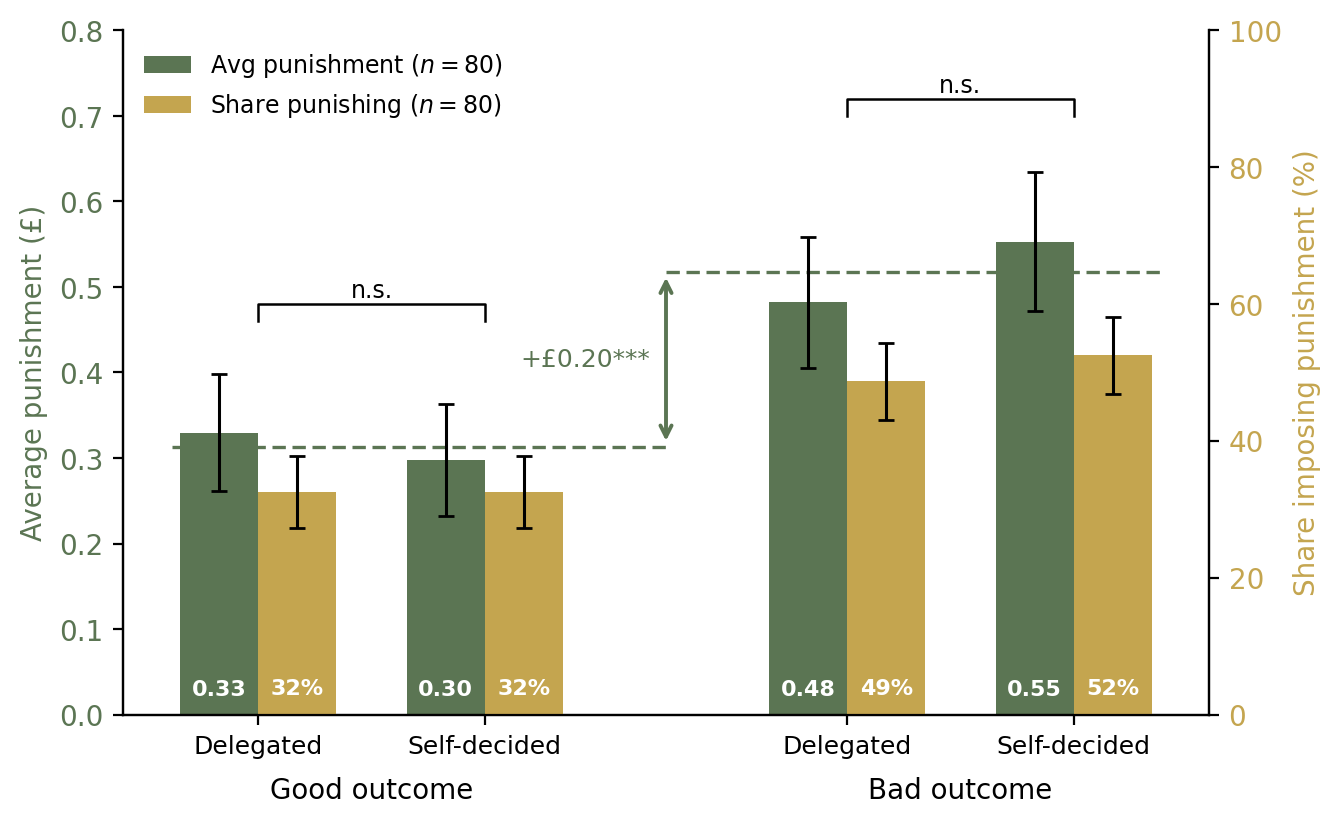
\includegraphics[width=0.75\linewidth]{../quality_reports/exhibits_excl_incredible_guessers/figures/punishment.png}
    \label{fig:excl_punishment}
\end{figure}

\clearpage
%% ---------------------------------------------------
%% reg_punishment  [IDENTICAL to live]   live location: results.tex:58
%% ---------------------------------------------------
\begin{table}[!htbp]
\centering
\scriptsize
\caption{Determinants of Player~B's chosen punishment}
\label{tab:excl_reg_punishment}
\begin{tabular}{@{\extracolsep{5pt}}lcc}
\\[-1.8ex]\hline
\hline \\[-1.8ex]
& \multicolumn{2}{c}{Dependent variable: \textit{Punishment (\pounds)}}\\[0.1cm]
& \textit{Full sample} & \textit{Passers} \\
\\[-1.8ex] & (1) & (2) \\
\hline \\[-1.8ex]
 Delegated & $0.032$ & $0.001$ \\
  & $(0.052)$ & $(0.054)$ \\[0.1cm]
 Bad outcome & $0.256^{***}$ & $0.260^{***}$ \\
  & $(0.071)$ & $(0.080)$ \\[0.1cm]
 Delegated $\times$ Bad outcome & $-0.103^{*}$ & $-0.078$ \\
  & $(0.058)$ & $(0.052)$ \\[0.1cm]
 Player B belief about Player A perf. & $-0.020$ & $0.001$ \\
  & $(0.032)$ & $(0.037)$ \\[0.1cm]
 Age & $0.002$ & $-0.001$ \\
  & $(0.005)$ & $(0.006)$ \\[0.1cm]
 Female & $-0.100$ & $-0.064$ \\
  & $(0.128)$ & $(0.140)$ \\[0.1cm]
 Socio-economic status & $0.083^{*}$ & $0.072$ \\
  & $(0.047)$ & $(0.049)$ \\[0.1cm]
 Went to uni & $-0.196$ & $-0.098$ \\
  & $(0.140)$ & $(0.142)$ \\[0.1cm]
 Technology score & $0.073$ & $0.030$ \\
  & $(0.053)$ & $(0.059)$ \\[0.1cm]
 Leadership position & $0.083$ & $0.061$ \\
  & $(0.142)$ & $(0.164)$ \\[0.1cm]
 Constant & $-0.077$ & $0.020$ \\
  & $(0.328)$ & $(0.374)$ \\[0.1cm]
\hline \\[-1.8ex]
 Observations & $320$ & $268$ \\
 Subjects & $80$ & $67$ \\
 Adj.\ $R^2$ & $0.077$ & $0.030$ \\
\hline
\hline \\[-1.8ex]
\multicolumn{3}{c}{\begin{minipage}{0.75\textwidth}\footnotesize \textit{Note:} OLS regression of Player~B's chosen punishment levels. The sample is stacked over the four (delegation, outcome) scenarios of the strategy method (4 observations per Player~B). Column~(1) uses the full Punishment-condition sample. Column~(2) restricts to Player~Bs who passed the attention check on the punishment-elicitation screen. Standard errors clustered at the Player~B level.\end{minipage}}
\end{tabular}
\end{table}

\clearpage

%% ---------------------------------------------------
%% realized_vs_anticipated  [IDENTICAL to live]   live location: results.tex:86
%% ---------------------------------------------------
\begin{figure}[!htbp]
    \centering
    \caption{Realized vs.\ anticipated punishment, by scenario}
    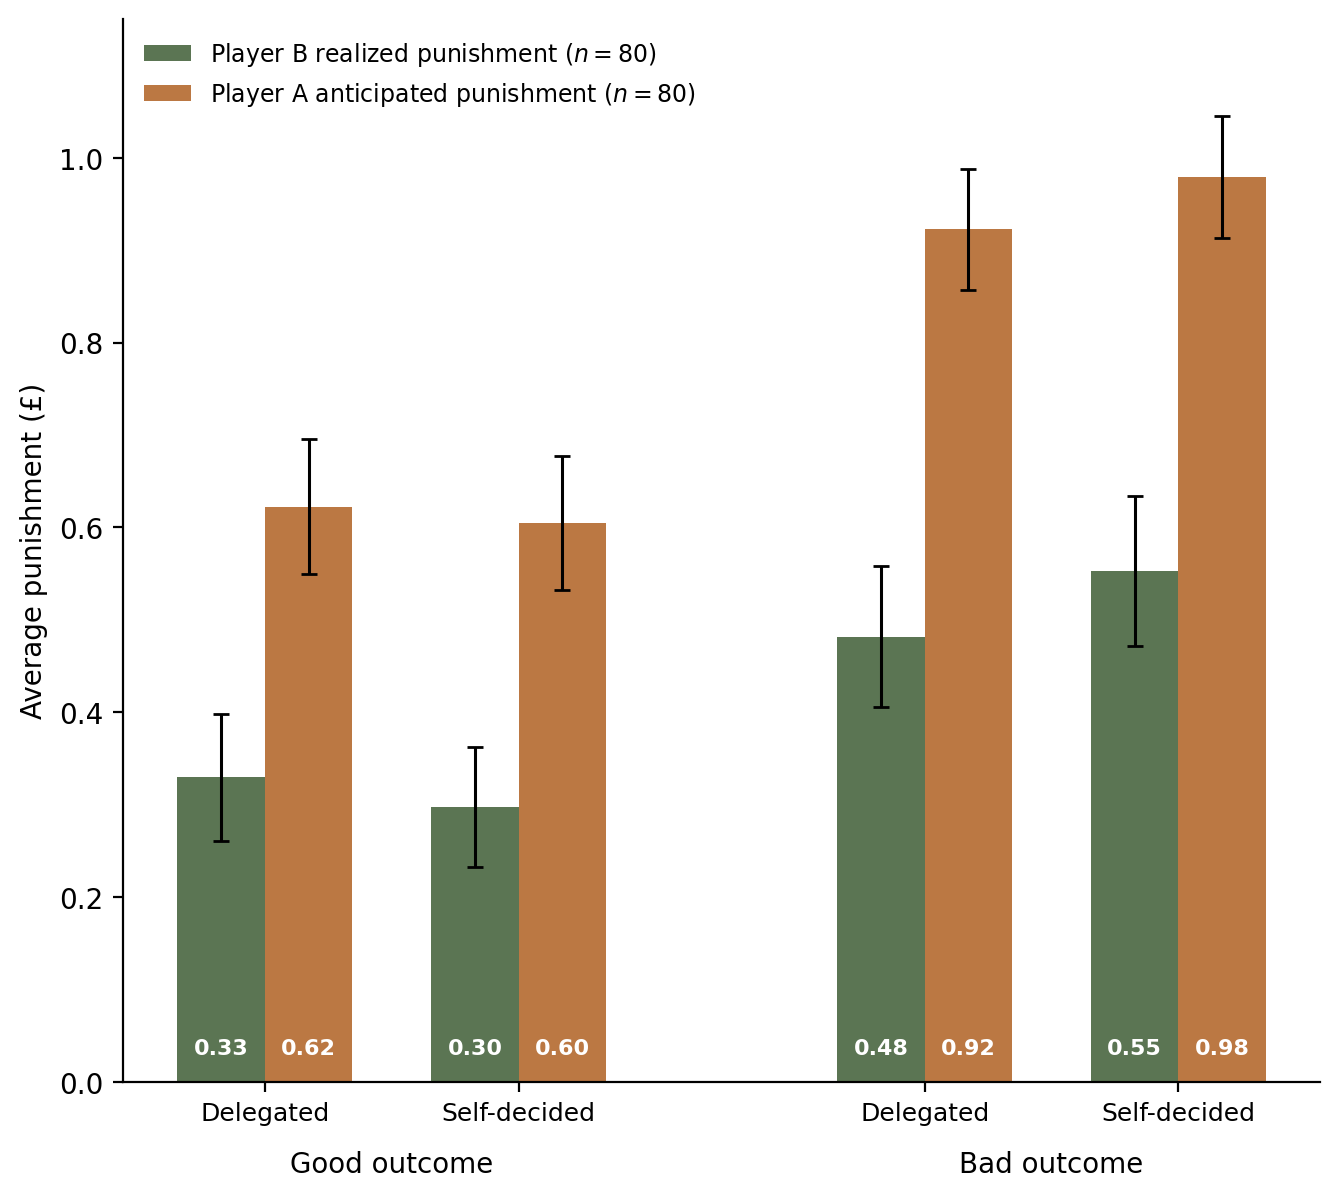
\includegraphics[width=0.75\linewidth]{../quality_reports/exhibits_excl_incredible_guessers/figures/realized_vs_anticipated.png}
    \label{fig:excl_realized_vs_anticipated}
\end{figure}

\clearpage

%% ---------------------------------------------------
%% reg_belief_specs  [IDENTICAL to live]   live location: results.tex:98
%% ---------------------------------------------------
\begin{table}[!htbp]
\centering
\scriptsize
\caption{Delegation and beliefs about punishment}
\label{tab:excl_reg_belief_specs}
\begin{tabular}{@{\extracolsep{5pt}}lcc|ccc}
\\[-1.8ex]\hline
\hline \\[-1.8ex]
& \multicolumn{5}{c}{Dependent variable: \textit{Delegation}}\\[0.1cm]
& \multicolumn{2}{c}{\textit{Full Punishment}} & \multicolumn{3}{c}{\textit{Punishment, passers}} \\
\\[-1.8ex] & (1) & (2) & (3) & (4) & (5) \\
\hline \\[-1.8ex]
 Belief difference, average ($\overline{\Delta}$) & $0.346$ & $0.398$ & $1.661^{**}$ &  &  \\
  & $(0.407)$ & $(0.448)$ & $(0.700)$ &  &  \\[0.1cm]
 Belief difference, weighted by $\Pr(\text{good})$ ($\Delta^{w}$) &  &  &  & $1.992^{**}$ &  \\
  &  &  &  & $(0.794)$ &  \\[0.1cm]
 Belief difference, bad outcome ($\Delta^{\text{bad}}$) &  &  &  &  & $0.590$ \\
  &  &  &  &  & $(0.424)$ \\[0.1cm]
 Belief difference, good outcome ($\Delta^{\text{good}}$) &  &  &  &  & $0.961^{**}$ \\
  &  &  &  &  & $(0.412)$ \\[0.1cm]
 Task performance &  & $-0.208^{*}$ & $-0.362^{***}$ & $-0.342^{**}$ & $-0.381^{***}$ \\
  &  & $(0.111)$ & $(0.136)$ & $(0.142)$ & $(0.138)$ \\[0.1cm]
 Age &  & $0.023^{*}$ & $0.039^{**}$ & $0.040^{**}$ & $0.039^{**}$ \\
  &  & $(0.012)$ & $(0.016)$ & $(0.016)$ & $(0.016)$ \\[0.1cm]
 Female &  & $0.152$ & $0.950^{**}$ & $1.026^{**}$ & $0.845^{*}$ \\
  &  & $(0.350)$ & $(0.427)$ & $(0.406)$ & $(0.444)$ \\[0.1cm]
 Socio-economic status &  & $-0.049$ & $-0.006$ & $-0.055$ & $0.001$ \\
  &  & $(0.111)$ & $(0.131)$ & $(0.133)$ & $(0.126)$ \\[0.1cm]
 Went to uni &  & $0.071$ & $-0.278$ & $-0.169$ & $-0.275$ \\
  &  & $(0.363)$ & $(0.412)$ & $(0.408)$ & $(0.409)$ \\[0.1cm]
 Technology score &  & $-0.061$ & $0.048$ & $0.072$ & $0.033$ \\
  &  & $(0.138)$ & $(0.170)$ & $(0.173)$ & $(0.167)$ \\[0.1cm]
 Leadership position &  & $0.302$ & $-0.301$ & $-0.279$ & $-0.245$ \\
  &  & $(0.312)$ & $(0.408)$ & $(0.408)$ & $(0.411)$ \\[0.1cm]
 Constant & $-0.198$ & $-0.345$ & $-1.228$ & $-1.281$ & $-1.115$ \\
  & $(0.142)$ & $(0.826)$ & $(1.155)$ & $(1.147)$ & $(1.165)$ \\[0.1cm]
\hline \\[-1.8ex]
 AME of belief measure (pp per \pounds 0.10) & $1.3$ & $1.4$ & $4.7^{**}$ & $5.5^{***}$ &  \\
  & $(p=0.388)$ & $(p=0.370)$ & $(p=0.011)$ & $(p=0.006)$ &  \\
 AME: good-outcome difference (pp per \pounds 0.10) &  &  &  &  & $2.7^{**}$ \\
  &  &  &  &  & $(p=0.010)$ \\
 AME: bad-outcome difference (pp per \pounds 0.10) &  &  &  &  & $1.7$ \\
  &  &  &  &  & $(p=0.165)$ \\
 Controls & $\times$ & \checkmark & \checkmark & \checkmark & \checkmark \\
 Passers only & $\times$ & $\times$ & \checkmark & \checkmark & \checkmark \\
 N & $80$ & $78$ & $60$ & $60$ & $60$ \\
 Pseudo $R^2$ & $0.007$ & $0.098$ & $0.248$ & $0.263$ & $0.252$ \\
\hline
\hline \\[-1.8ex]
\multicolumn{6}{c}{\begin{minipage}{0.92\textwidth}\footnotesize \textit{Note:} Probit estimates with robust (HC1) standard errors in parentheses. Sample restricted to the \textit{Punishment} condition throughout. Belief differences are within-subject \textit{(no delegation)}~$-$~\textit{(delegation)} in expected punishment, so positive coefficients indicate that subjects who expect to be punished more harshly for not delegating (relative to delegating) are more likely to delegate. Columns~(1)--(3) use the simple average of the good-outcome and the bad-outcome belief difference. Column~(4) instead weights the good-outcome difference by Player~A's elicited probability of producing the high payoff and the bad-outcome difference by the complementary probability. Column~(5) enters the two differences separately. The \textit{AME} rows report the average marginal effect of the belief measure entered in the respective column on the probability of delegation, in percentage points per \pounds 0.10 increase in the corresponding belief difference.\end{minipage}}
\end{tabular}
\end{table}

\clearpage

%% ---------------------------------------------------
%% performance_overview  [CHANGED]   live location: results.tex:121
%% ---------------------------------------------------
\begin{figure}[!htbp]
    \centering
    \caption{Delegation, performance, and confidence by condition}
    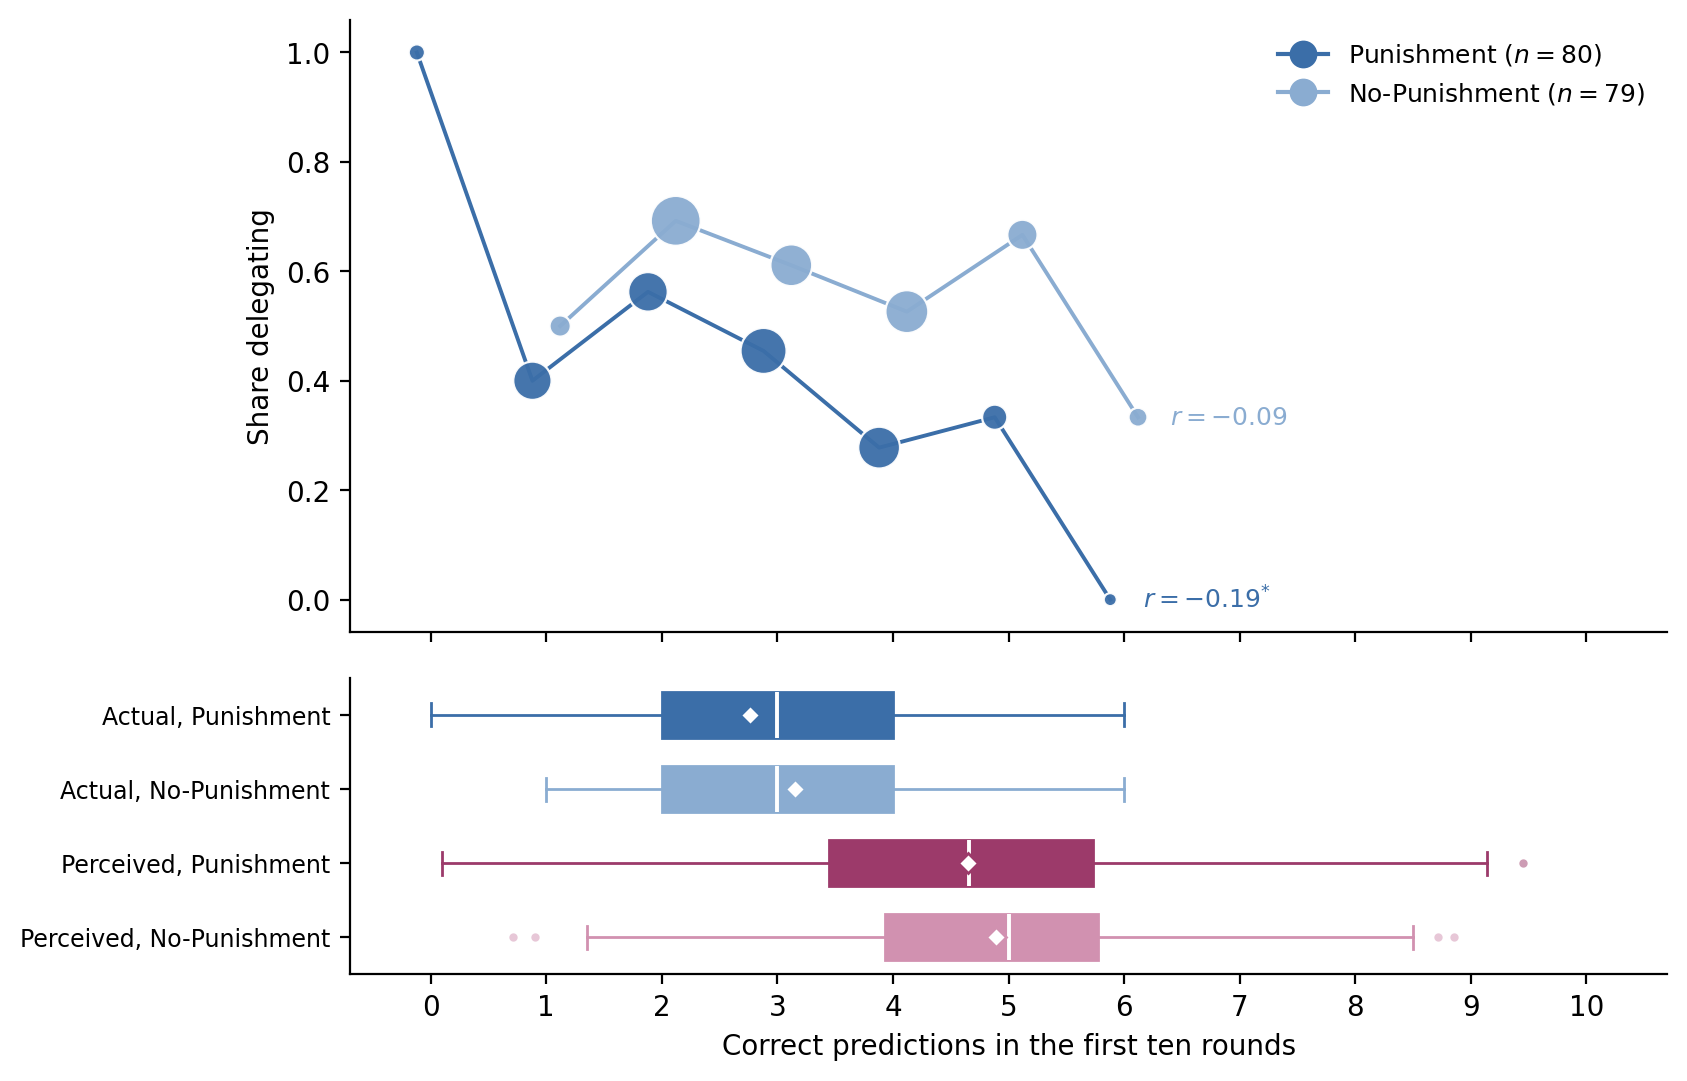
\includegraphics[width=0.9\linewidth]{../quality_reports/exhibits_excl_incredible_guessers/figures/performance_overview.png}
    \label{fig:excl_performance_overview}
\end{figure}

\clearpage

\clearpage
\subsection*{Appendix}

%% ---------------------------------------------------
%% balance_player_a  [CHANGED]   live location: appendix.tex:9
%% ---------------------------------------------------
\begin{table}[!htbp]
    \centering
    \caption{Condition balance --- Player~A}
    \label{tab:excl_treatment_balance}
    \begin{tabular}{l|rrr}
                  Variable &  \textit{Punishment} &  \textit{No-Punishment} &  $p$-value \\ \hline
                           Age &  $39.026$ &  $37.886$ &  $0.557$ \\
                        Female &  $0.487$ &  $0.506$ &  $0.936$ \\
         Socio-economic status &  $5.179$ &  $5.329$ &  $0.542$ \\
                   Went to uni &  $0.575$ &  $0.557$ &  $0.945$ \\
              Technology score &  $2.087$ &  $2.266$ &  $0.366$ \\
           Leadership position &  $0.362$ &  $0.329$ &  $0.783$ \\
    \end{tabular}
    \begin{minipage}{0.95\textwidth}\footnotesize
    \textit{Note:} Mean values by condition for Player~A, with $p$-values from two-sided $t$-tests for continuous variables and Chi-squared tests for binary variables. \textit{Socio-economic status} is self-reported on a $1$--$10$ scale. \textit{Went to uni} indicates a university degree. \textit{Technology score} is constructed from weekly device usage, programming skills, cryptocurrency knowledge, technology use at work, and similar items. \textit{Leadership position} indicates self-reported management or supervisory experience.
    \end{minipage}
\end{table}

\clearpage

%% ---------------------------------------------------
%% reg_punishment_extensive  [IDENTICAL to live]   live location: appendix.tex:19
%% ---------------------------------------------------
\begin{table}[!htbp]
\centering
\scriptsize
\caption{Extensive margin of punishment --- probit for $\Pr(\text{punishment}>0)$}
\label{tab:excl_reg_punishment_extensive}
\begin{tabular}{@{\extracolsep{5pt}}lcc}
\\[-1.8ex]\hline
\hline \\[-1.8ex]
& \multicolumn{2}{c}{Dependent variable: \textit{Any punishment}}\\[0.1cm]
& \textit{Full sample} & \textit{Passers} \\
\\[-1.8ex] & (1) & (2) \\
\hline \\[-1.8ex]
 Delegated & $0.002$ & $-0.042$ \\
  & $(0.077)$ & $(0.078)$ \\[0.1cm]
 Bad outcome & $0.556^{***}$ & $0.563^{***}$ \\
  & $(0.139)$ & $(0.153)$ \\[0.1cm]
 Delegated $\times$ Bad outcome & $-0.099$ & $-0.072$ \\
  & $(0.095)$ & $(0.103)$ \\[0.1cm]
 Player B belief about Player A perf. & $-0.083$ & $-0.030$ \\
  & $(0.075)$ & $(0.082)$ \\[0.1cm]
 Age & $-0.006$ & $-0.013$ \\
  & $(0.013)$ & $(0.015)$ \\[0.1cm]
 Female & $0.115$ & $0.230$ \\
  & $(0.272)$ & $(0.291)$ \\[0.1cm]
 Socio-economic status & $0.160$ & $0.140$ \\
  & $(0.126)$ & $(0.129)$ \\[0.1cm]
 Went to uni & $-0.827^{***}$ & $-0.706^{**}$ \\
  & $(0.320)$ & $(0.349)$ \\[0.1cm]
 Technology score & $0.062$ & $-0.023$ \\
  & $(0.118)$ & $(0.131)$ \\[0.1cm]
 Leadership position & $0.062$ & $-0.071$ \\
  & $(0.293)$ & $(0.321)$ \\[0.1cm]
 Constant & $-0.382$ & $-0.182$ \\
  & $(0.807)$ & $(0.864)$ \\[0.1cm]
\hline \\[-1.8ex]
 AME of Delegated (pp) & $-1.8$ & $-2.9$ \\
  & $(p=0.462)$ & $(p=0.285)$ \\
 AME of Bad outcome (pp) & $18.1^{***}$ & $19.4^{***}$ \\
  & $(p<0.001)$ & $(p<0.001)$ \\
 Observations & $320$ & $268$ \\
 Subjects & $80$ & $67$ \\
 Pseudo $R^2$ & $0.096$ & $0.081$ \\
\hline
\hline \\[-1.8ex]
\multicolumn{3}{c}{\begin{minipage}{0.85\textwidth}\footnotesize \textit{Note:} Probit regression of an indicator for non-zero punishment ($1\{\text{punishment}>0\}$) on a delegation indicator, a bad-outcome indicator, their interaction, Player~B's belief about Player~A's performance, and socio-demographic controls; the sample is stacked over the four (delegation, outcome) cells of the strategy method (4 observations per Player~B). Column~(1) uses the full Punishment-condition sample; Column~(2) restricts to attention-check passers. Standard errors clustered at the Player~B level. The \textit{AME} rows report discrete average marginal effects on the probability of imposing any punishment, in percentage points (for Delegated, the change from $0\to1$ with the interaction moved consistently; for Bad outcome, likewise), computed by counterfactual prediction with p-values from a seeded $400$-replication subject-cluster bootstrap. Significance: $^{*}\,p<0.10$; $^{**}\,p<0.05$; $^{***}\,p<0.01$ (two-sided).\end{minipage}}
\end{tabular}
\end{table}

\clearpage

%% ---------------------------------------------------
%% punishment_passers  [IDENTICAL to live]   live location: appendix.tex:56
%% ---------------------------------------------------
\begin{figure}[!htbp]
    \centering
    \caption{Player~B punishment by delegation and outcome scenario, attention-check passers}
    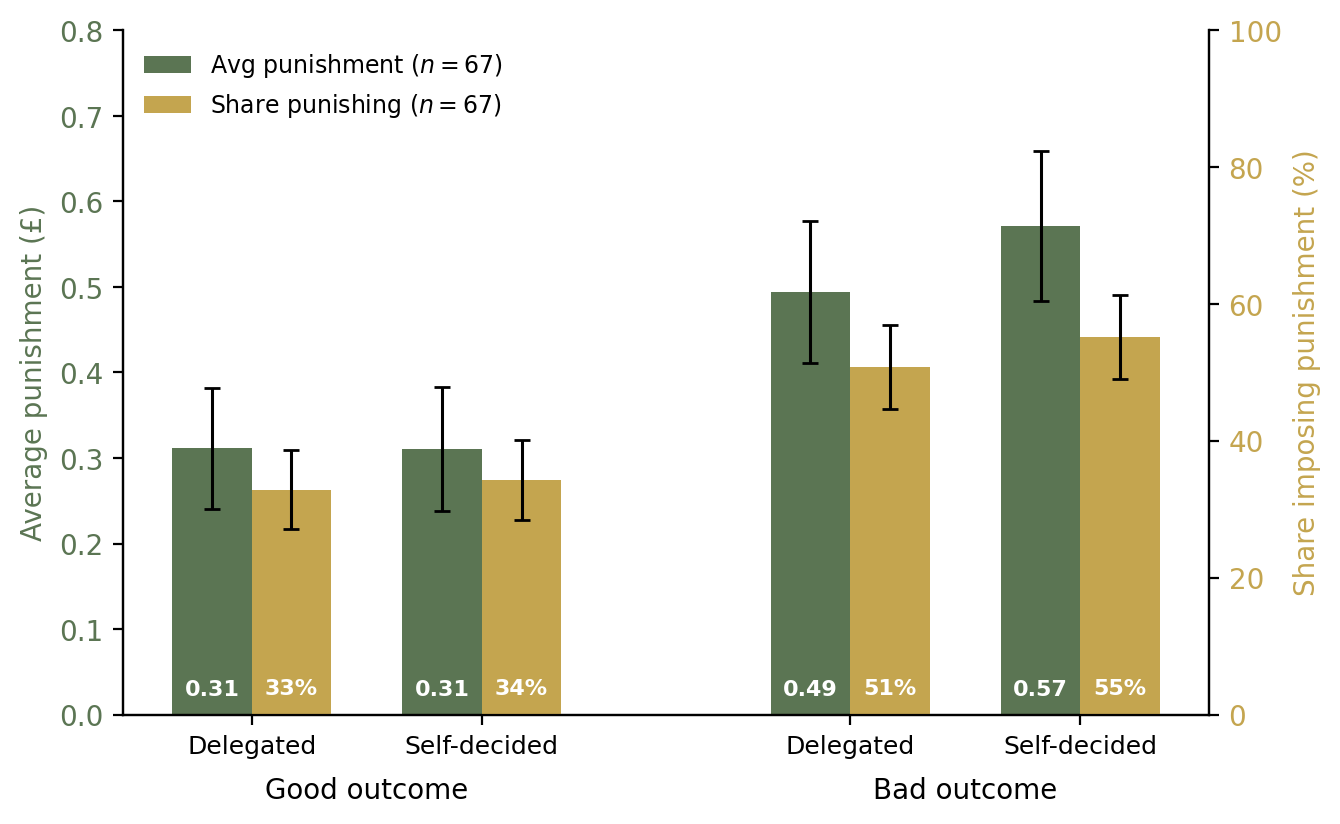
\includegraphics[width=0.65\linewidth]{../quality_reports/exhibits_excl_incredible_guessers/figures/punishment_passers.png}
    \label{fig:excl_punishment_passers}
\end{figure}

\clearpage

%% ---------------------------------------------------
%% realized_vs_anticipated_passers  [IDENTICAL to live]   live location: appendix.tex:67
%% ---------------------------------------------------
\begin{figure}[!htbp]
    \centering
    \caption{Realized vs.\ anticipated punishment, attention-check passers}
    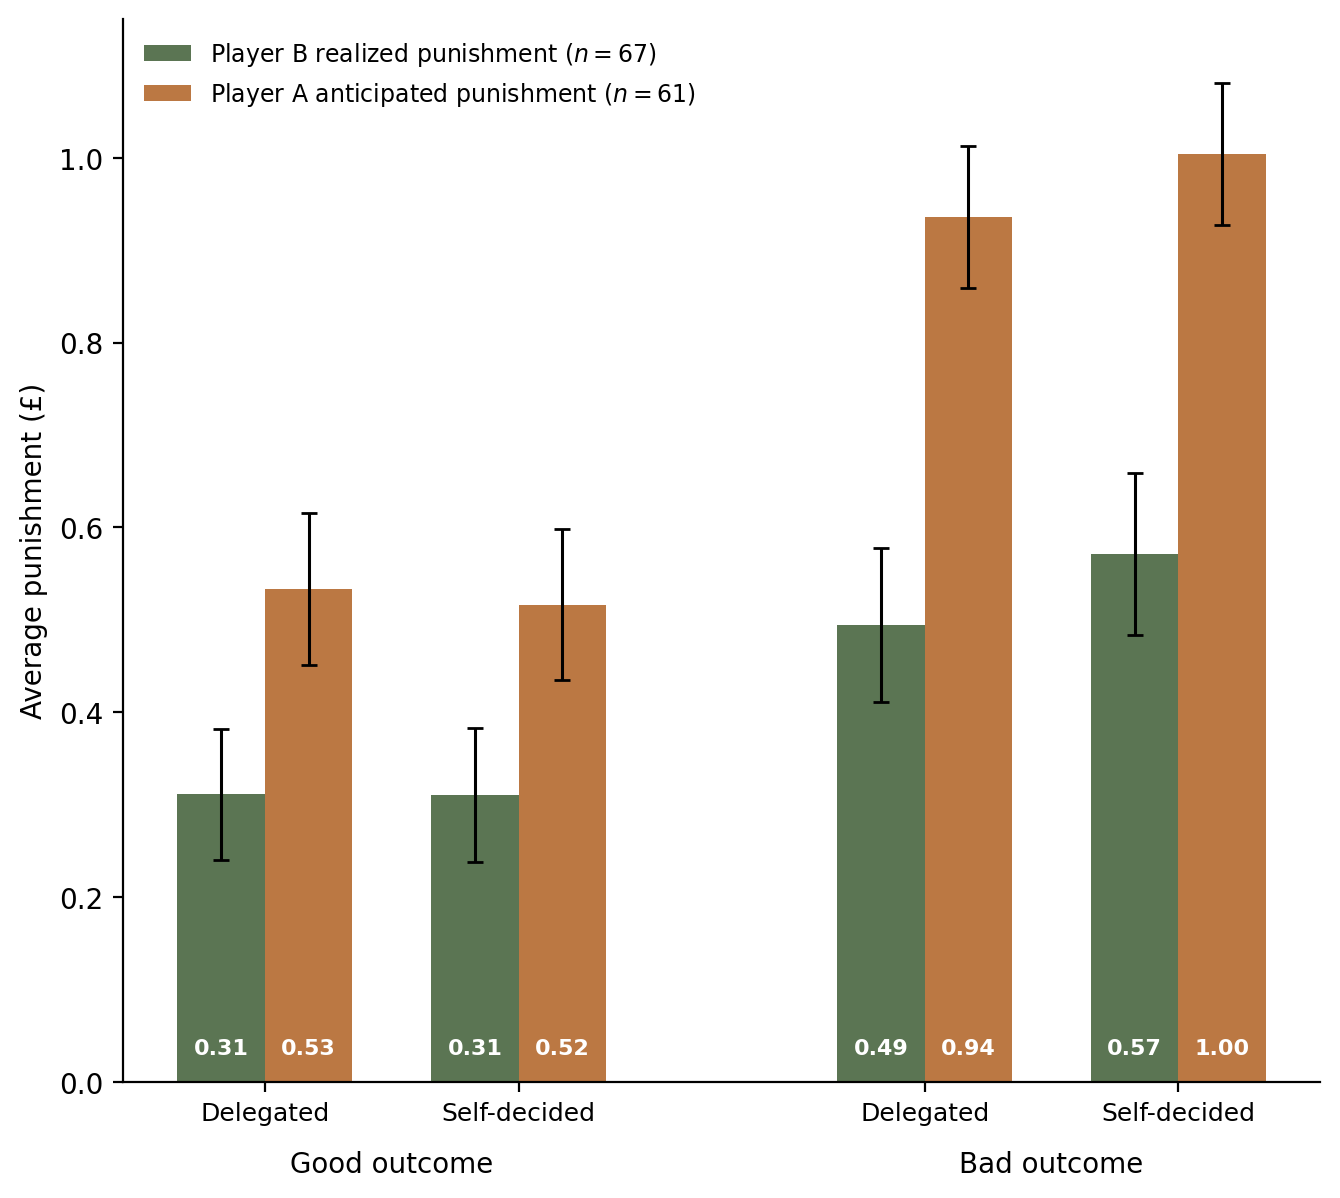
\includegraphics[width=0.75\linewidth]{../quality_reports/exhibits_excl_incredible_guessers/figures/realized_vs_anticipated_passers.png}
    \label{fig:excl_realized_vs_anticipated_passers}
\end{figure}

\clearpage

%% ---------------------------------------------------
%% punishment_hypothetical  [CHANGED]   live location: appendix.tex:83
%% ---------------------------------------------------
\begin{figure}[!htbp]
    \centering
    \caption{Hypothetical punishment by delegation and outcome scenario (\textit{No-Punishment} condition)}
    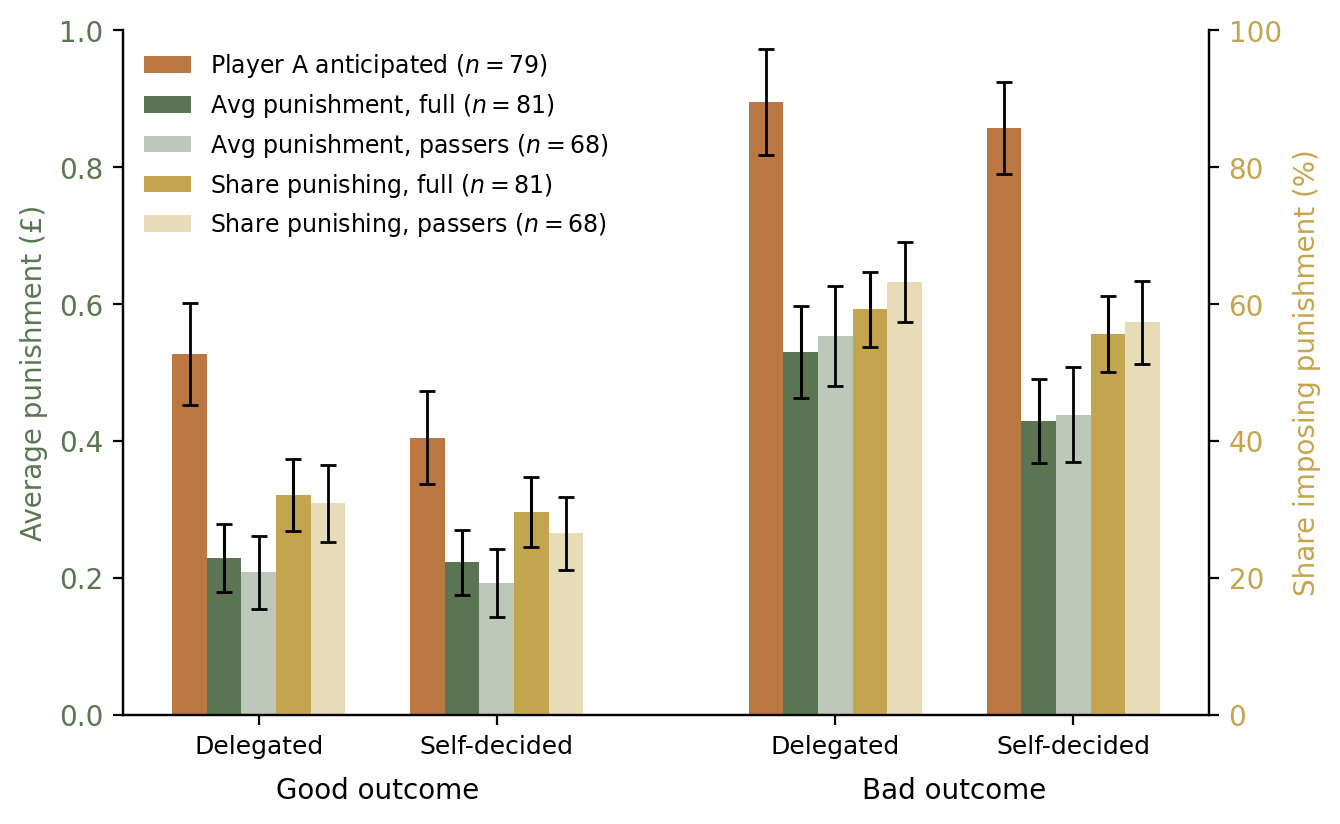
\includegraphics[width=0.65\linewidth]{../quality_reports/exhibits_excl_incredible_guessers/figures/punishment_hypothetical.png}
    \label{fig:excl_punishment_hypothetical}
\end{figure}

\clearpage

%%  from manuscript/main.tex. Every label carries an excl_ prefix, so this
%%  file can coexist with the live exhibits in a single document.
%% =====================================================================

\clearpage
\section*{Exhibits excluding the two incredible weight guessers}

\clearpage
\subsection*{Results}

%% ---------------------------------------------------
%% delegation_shares  [CHANGED]   live location: results.tex:19
%% ---------------------------------------------------
\begin{figure}[!htbp]
    \centering
    \caption{Delegation shares by condition}
    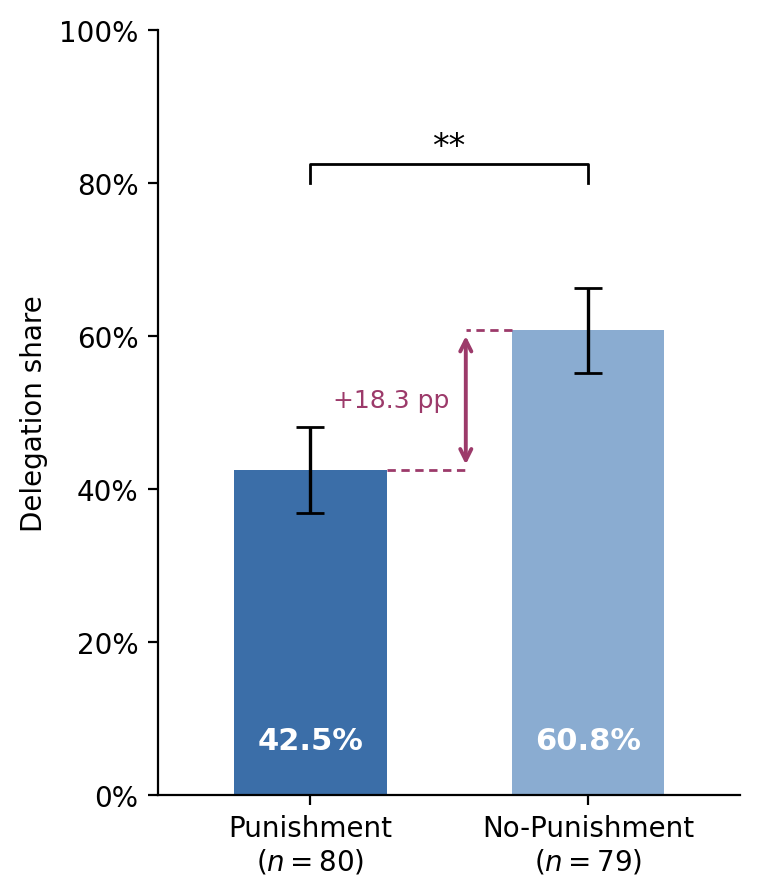
\includegraphics[width=0.5\linewidth]{../quality_reports/exhibits_excl_incredible_guessers/figures/delegation_shares.png}
    \label{fig:excl_delegation_shares}
\end{figure}

\clearpage
%% ---------------------------------------------------
%% reg_delegation  [CHANGED]   live location: results.tex:31
%% ---------------------------------------------------
\begin{table}[!htbp]
\centering
\scriptsize
\caption{Determinants of the delegation decision}
\label{tab:excl_del_decision_determinants}
\begin{tabular}{@{\extracolsep{5pt}}lcccc|c}
\\[-1.8ex]\hline
\hline \\[-1.8ex]
& \multicolumn{5}{c}{Dependent variable: \textit{Delegation}}\\[0.1cm]
& \multicolumn{4}{c}{\textit{Full sample}} & \textit{Passers} \\
\\[-1.8ex] & (1) & (2) & (3) & (4) & (5) \\
\hline \\[-1.8ex]
 Punishment indicator & $-0.462^{**}$ & $-0.473^{**}$ & $-0.537^{**}$ & $-0.489^{**}$ & $-0.589^{**}$ \\
  & $(0.201)$ & $(0.206)$ & $(0.209)$ & $(0.207)$ & $(0.235)$ \\[0.1cm]
 Task performance &  &  & $-0.160^{**}$ &  & $-0.203^{**}$ \\
  &  &  & $(0.081)$ &  & $(0.089)$ \\[0.1cm]
 Perceived performance &  &  &  & $-0.075$ &  \\
  &  &  &  & $(0.057)$ &  \\[0.1cm]
 Age &  & $-0.003$ & $-0.002$ & $-0.002$ & $0.002$ \\
  &  & $(0.009)$ & $(0.009)$ & $(0.009)$ & $(0.011)$ \\[0.1cm]
 Female &  & $0.141$ & $0.194$ & $0.181$ & $0.372$ \\
  &  & $(0.228)$ & $(0.230)$ & $(0.231)$ & $(0.257)$ \\[0.1cm]
 Socio-economic status &  & $-0.044$ & $-0.042$ & $-0.036$ & $-0.086$ \\
  &  & $(0.071)$ & $(0.073)$ & $(0.072)$ & $(0.081)$ \\[0.1cm]
 Went to uni &  & $0.032$ & $0.062$ & $0.020$ & $0.118$ \\
  &  & $(0.228)$ & $(0.226)$ & $(0.227)$ & $(0.248)$ \\[0.1cm]
 Technology score &  & $-0.065$ & $-0.036$ & $-0.056$ & $0.024$ \\
  &  & $(0.093)$ & $(0.096)$ & $(0.093)$ & $(0.109)$ \\[0.1cm]
 Leadership position &  & $0.415^{*}$ & $0.444^{*}$ & $0.411^{*}$ & $0.278$ \\
  &  & $(0.226)$ & $(0.228)$ & $(0.226)$ & $(0.256)$ \\[0.1cm]
 Constant & $0.273^{*}$ & $0.533$ & $0.908$ & $0.801$ & $0.851$ \\
  & $(0.143)$ & $(0.557)$ & $(0.593)$ & $(0.606)$ & $(0.673)$ \\[0.1cm]
\hline \\[-1.8ex]
 AME of Punishment (pp) & $-18.3^{**}$ & $-18.3^{**}$ & $-20.3^{***}$ & $-18.7^{**}$ & $-21.8^{***}$ \\
  & $(p=0.019)$ & $(p=0.019)$ & $(p=0.008)$ & $(p=0.016)$ & $(p=0.009)$ \\
 N & $159$ & $157$ & $157$ & $157$ & $128$ \\
 Pseudo $R^2$ & $0.024$ & $0.042$ & $0.060$ & $0.051$ & $0.077$ \\
\hline
\hline \\[-1.8ex]
\multicolumn{6}{c}{\begin{minipage}{0.85\textwidth}\footnotesize \textit{Note:} Coefficients from a Probit regression of the delegation decision on the Punishment indicator and a set of controls. Robust (HC1) standard errors in parentheses. Significance: $^{*}\,p<0.10$; $^{**}\,p<0.05$; $^{***}\,p<0.01$ (two-sided). Due to missing socio-demographic data, two subjects are dropped in Columns~(2)--(5). The \textit{AME of Punishment} reports the average change in the predicted probability of delegation from introducing the punishment possibility, in percentage points.\end{minipage}}
\end{tabular}
\end{table}

\clearpage

%% ---------------------------------------------------
%% punishment  [IDENTICAL to live]   live location: results.tex:40
%% ---------------------------------------------------
\begin{figure}[!htbp]
    \centering
    \caption{Player~B punishment by delegation and outcome scenario}
    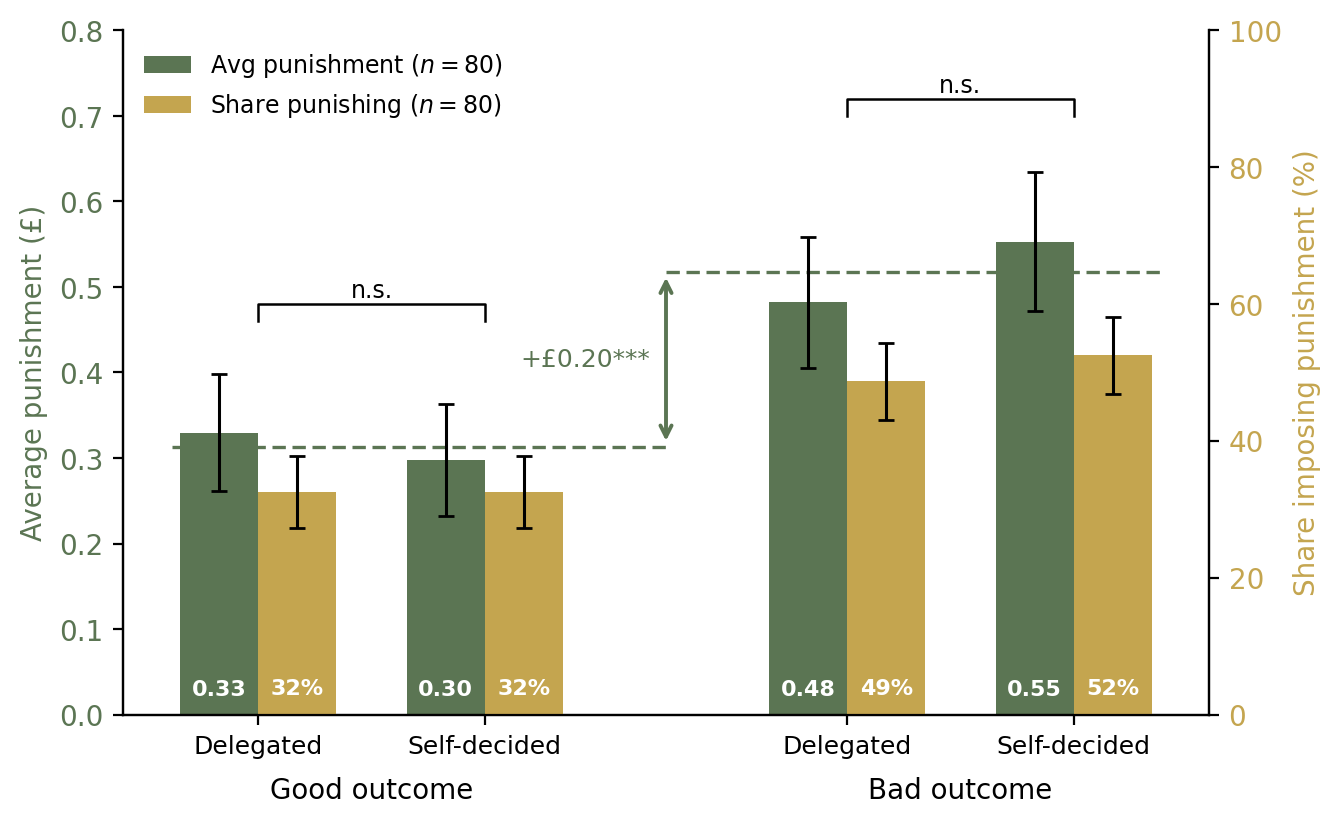
\includegraphics[width=0.75\linewidth]{../quality_reports/exhibits_excl_incredible_guessers/figures/punishment.png}
    \label{fig:excl_punishment}
\end{figure}

\clearpage
%% ---------------------------------------------------
%% reg_punishment  [IDENTICAL to live]   live location: results.tex:58
%% ---------------------------------------------------
\begin{table}[!htbp]
\centering
\scriptsize
\caption{Determinants of Player~B's chosen punishment}
\label{tab:excl_reg_punishment}
\begin{tabular}{@{\extracolsep{5pt}}lcc}
\\[-1.8ex]\hline
\hline \\[-1.8ex]
& \multicolumn{2}{c}{Dependent variable: \textit{Punishment (\pounds)}}\\[0.1cm]
& \textit{Full sample} & \textit{Passers} \\
\\[-1.8ex] & (1) & (2) \\
\hline \\[-1.8ex]
 Delegated & $0.032$ & $0.001$ \\
  & $(0.052)$ & $(0.054)$ \\[0.1cm]
 Bad outcome & $0.256^{***}$ & $0.260^{***}$ \\
  & $(0.071)$ & $(0.080)$ \\[0.1cm]
 Delegated $\times$ Bad outcome & $-0.103^{*}$ & $-0.078$ \\
  & $(0.058)$ & $(0.052)$ \\[0.1cm]
 Player B belief about Player A perf. & $-0.020$ & $0.001$ \\
  & $(0.032)$ & $(0.037)$ \\[0.1cm]
 Age & $0.002$ & $-0.001$ \\
  & $(0.005)$ & $(0.006)$ \\[0.1cm]
 Female & $-0.100$ & $-0.064$ \\
  & $(0.128)$ & $(0.140)$ \\[0.1cm]
 Socio-economic status & $0.083^{*}$ & $0.072$ \\
  & $(0.047)$ & $(0.049)$ \\[0.1cm]
 Went to uni & $-0.196$ & $-0.098$ \\
  & $(0.140)$ & $(0.142)$ \\[0.1cm]
 Technology score & $0.073$ & $0.030$ \\
  & $(0.053)$ & $(0.059)$ \\[0.1cm]
 Leadership position & $0.083$ & $0.061$ \\
  & $(0.142)$ & $(0.164)$ \\[0.1cm]
 Constant & $-0.077$ & $0.020$ \\
  & $(0.328)$ & $(0.374)$ \\[0.1cm]
\hline \\[-1.8ex]
 Observations & $320$ & $268$ \\
 Subjects & $80$ & $67$ \\
 Adj.\ $R^2$ & $0.077$ & $0.030$ \\
\hline
\hline \\[-1.8ex]
\multicolumn{3}{c}{\begin{minipage}{0.75\textwidth}\footnotesize \textit{Note:} OLS regression of Player~B's chosen punishment levels. The sample is stacked over the four (delegation, outcome) scenarios of the strategy method (4 observations per Player~B). Column~(1) uses the full Punishment-condition sample. Column~(2) restricts to Player~Bs who passed the attention check on the punishment-elicitation screen. Standard errors clustered at the Player~B level.\end{minipage}}
\end{tabular}
\end{table}

\clearpage

%% ---------------------------------------------------
%% realized_vs_anticipated  [IDENTICAL to live]   live location: results.tex:86
%% ---------------------------------------------------
\begin{figure}[!htbp]
    \centering
    \caption{Realized vs.\ anticipated punishment, by scenario}
    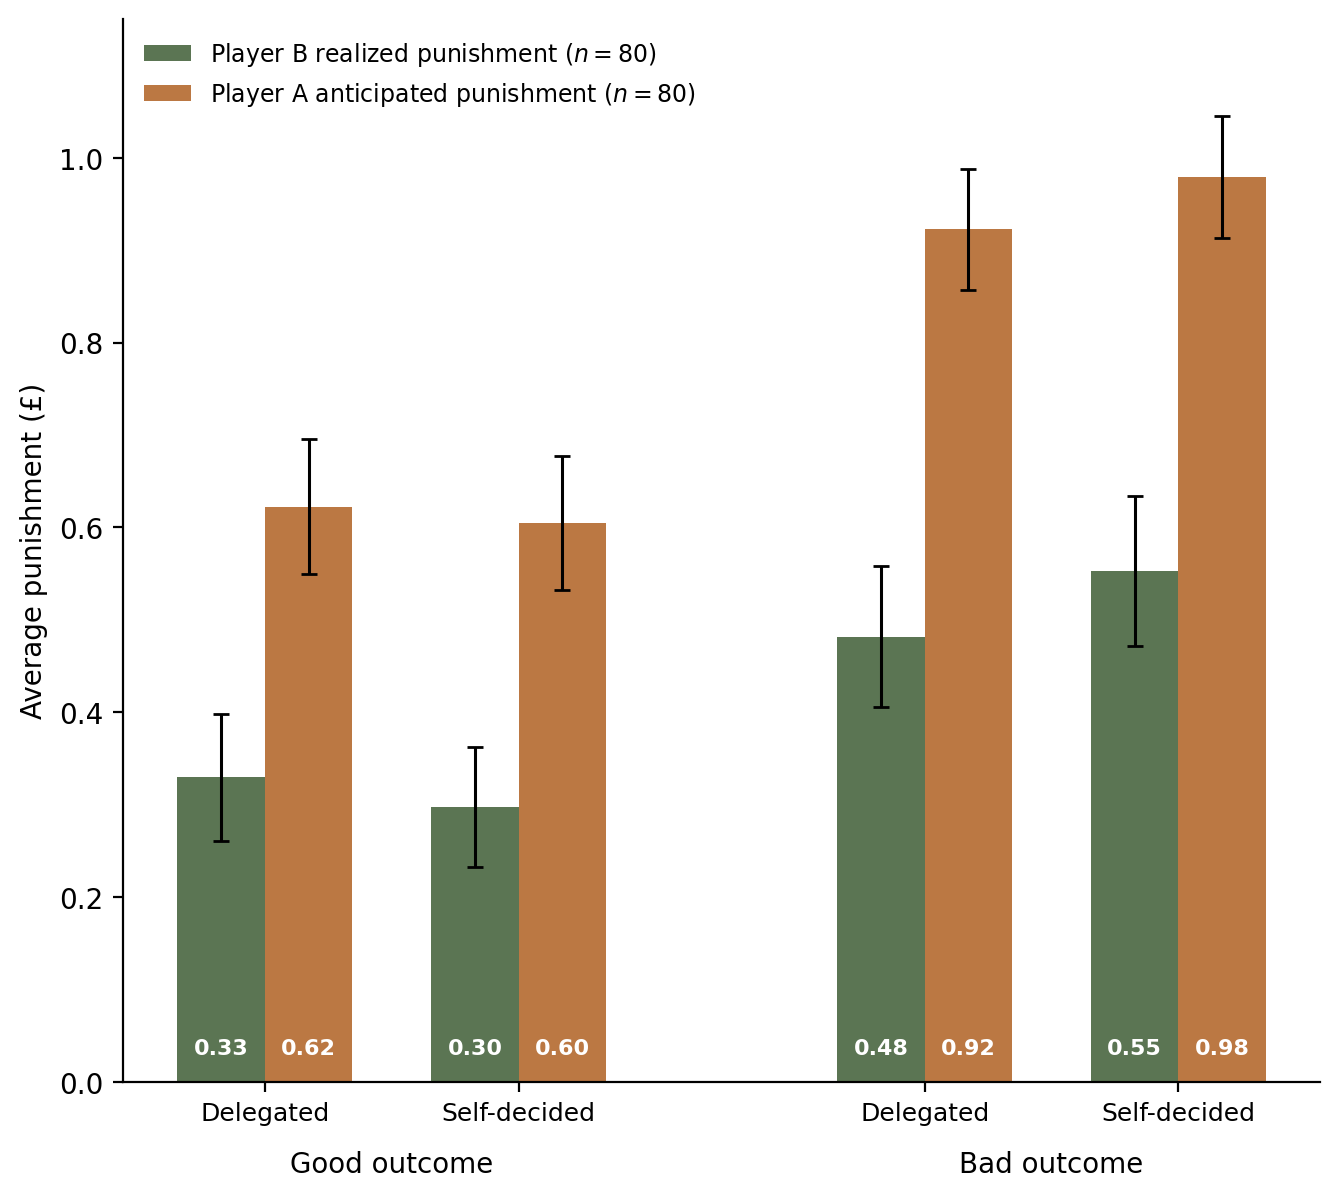
\includegraphics[width=0.75\linewidth]{../quality_reports/exhibits_excl_incredible_guessers/figures/realized_vs_anticipated.png}
    \label{fig:excl_realized_vs_anticipated}
\end{figure}

\clearpage

%% ---------------------------------------------------
%% reg_belief_specs  [IDENTICAL to live]   live location: results.tex:98
%% ---------------------------------------------------
\begin{table}[!htbp]
\centering
\scriptsize
\caption{Delegation and beliefs about punishment}
\label{tab:excl_reg_belief_specs}
\begin{tabular}{@{\extracolsep{5pt}}lcc|ccc}
\\[-1.8ex]\hline
\hline \\[-1.8ex]
& \multicolumn{5}{c}{Dependent variable: \textit{Delegation}}\\[0.1cm]
& \multicolumn{2}{c}{\textit{Full Punishment}} & \multicolumn{3}{c}{\textit{Punishment, passers}} \\
\\[-1.8ex] & (1) & (2) & (3) & (4) & (5) \\
\hline \\[-1.8ex]
 Belief difference, average ($\overline{\Delta}$) & $0.346$ & $0.398$ & $1.661^{**}$ &  &  \\
  & $(0.407)$ & $(0.448)$ & $(0.700)$ &  &  \\[0.1cm]
 Belief difference, weighted by $\Pr(\text{good})$ ($\Delta^{w}$) &  &  &  & $1.992^{**}$ &  \\
  &  &  &  & $(0.794)$ &  \\[0.1cm]
 Belief difference, bad outcome ($\Delta^{\text{bad}}$) &  &  &  &  & $0.590$ \\
  &  &  &  &  & $(0.424)$ \\[0.1cm]
 Belief difference, good outcome ($\Delta^{\text{good}}$) &  &  &  &  & $0.961^{**}$ \\
  &  &  &  &  & $(0.412)$ \\[0.1cm]
 Task performance &  & $-0.208^{*}$ & $-0.362^{***}$ & $-0.342^{**}$ & $-0.381^{***}$ \\
  &  & $(0.111)$ & $(0.136)$ & $(0.142)$ & $(0.138)$ \\[0.1cm]
 Age &  & $0.023^{*}$ & $0.039^{**}$ & $0.040^{**}$ & $0.039^{**}$ \\
  &  & $(0.012)$ & $(0.016)$ & $(0.016)$ & $(0.016)$ \\[0.1cm]
 Female &  & $0.152$ & $0.950^{**}$ & $1.026^{**}$ & $0.845^{*}$ \\
  &  & $(0.350)$ & $(0.427)$ & $(0.406)$ & $(0.444)$ \\[0.1cm]
 Socio-economic status &  & $-0.049$ & $-0.006$ & $-0.055$ & $0.001$ \\
  &  & $(0.111)$ & $(0.131)$ & $(0.133)$ & $(0.126)$ \\[0.1cm]
 Went to uni &  & $0.071$ & $-0.278$ & $-0.169$ & $-0.275$ \\
  &  & $(0.363)$ & $(0.412)$ & $(0.408)$ & $(0.409)$ \\[0.1cm]
 Technology score &  & $-0.061$ & $0.048$ & $0.072$ & $0.033$ \\
  &  & $(0.138)$ & $(0.170)$ & $(0.173)$ & $(0.167)$ \\[0.1cm]
 Leadership position &  & $0.302$ & $-0.301$ & $-0.279$ & $-0.245$ \\
  &  & $(0.312)$ & $(0.408)$ & $(0.408)$ & $(0.411)$ \\[0.1cm]
 Constant & $-0.198$ & $-0.345$ & $-1.228$ & $-1.281$ & $-1.115$ \\
  & $(0.142)$ & $(0.826)$ & $(1.155)$ & $(1.147)$ & $(1.165)$ \\[0.1cm]
\hline \\[-1.8ex]
 AME of belief measure (pp per \pounds 0.10) & $1.3$ & $1.4$ & $4.7^{**}$ & $5.5^{***}$ &  \\
  & $(p=0.388)$ & $(p=0.370)$ & $(p=0.011)$ & $(p=0.006)$ &  \\
 AME: good-outcome difference (pp per \pounds 0.10) &  &  &  &  & $2.7^{**}$ \\
  &  &  &  &  & $(p=0.010)$ \\
 AME: bad-outcome difference (pp per \pounds 0.10) &  &  &  &  & $1.7$ \\
  &  &  &  &  & $(p=0.165)$ \\
 Controls & $\times$ & \checkmark & \checkmark & \checkmark & \checkmark \\
 Passers only & $\times$ & $\times$ & \checkmark & \checkmark & \checkmark \\
 N & $80$ & $78$ & $60$ & $60$ & $60$ \\
 Pseudo $R^2$ & $0.007$ & $0.098$ & $0.248$ & $0.263$ & $0.252$ \\
\hline
\hline \\[-1.8ex]
\multicolumn{6}{c}{\begin{minipage}{0.92\textwidth}\footnotesize \textit{Note:} Probit estimates with robust (HC1) standard errors in parentheses. Sample restricted to the \textit{Punishment} condition throughout. Belief differences are within-subject \textit{(no delegation)}~$-$~\textit{(delegation)} in expected punishment, so positive coefficients indicate that subjects who expect to be punished more harshly for not delegating (relative to delegating) are more likely to delegate. Columns~(1)--(3) use the simple average of the good-outcome and the bad-outcome belief difference. Column~(4) instead weights the good-outcome difference by Player~A's elicited probability of producing the high payoff and the bad-outcome difference by the complementary probability. Column~(5) enters the two differences separately. The \textit{AME} rows report the average marginal effect of the belief measure entered in the respective column on the probability of delegation, in percentage points per \pounds 0.10 increase in the corresponding belief difference.\end{minipage}}
\end{tabular}
\end{table}

\clearpage

%% ---------------------------------------------------
%% performance_overview  [CHANGED]   live location: results.tex:121
%% ---------------------------------------------------
\begin{figure}[!htbp]
    \centering
    \caption{Delegation, performance, and confidence by condition}
    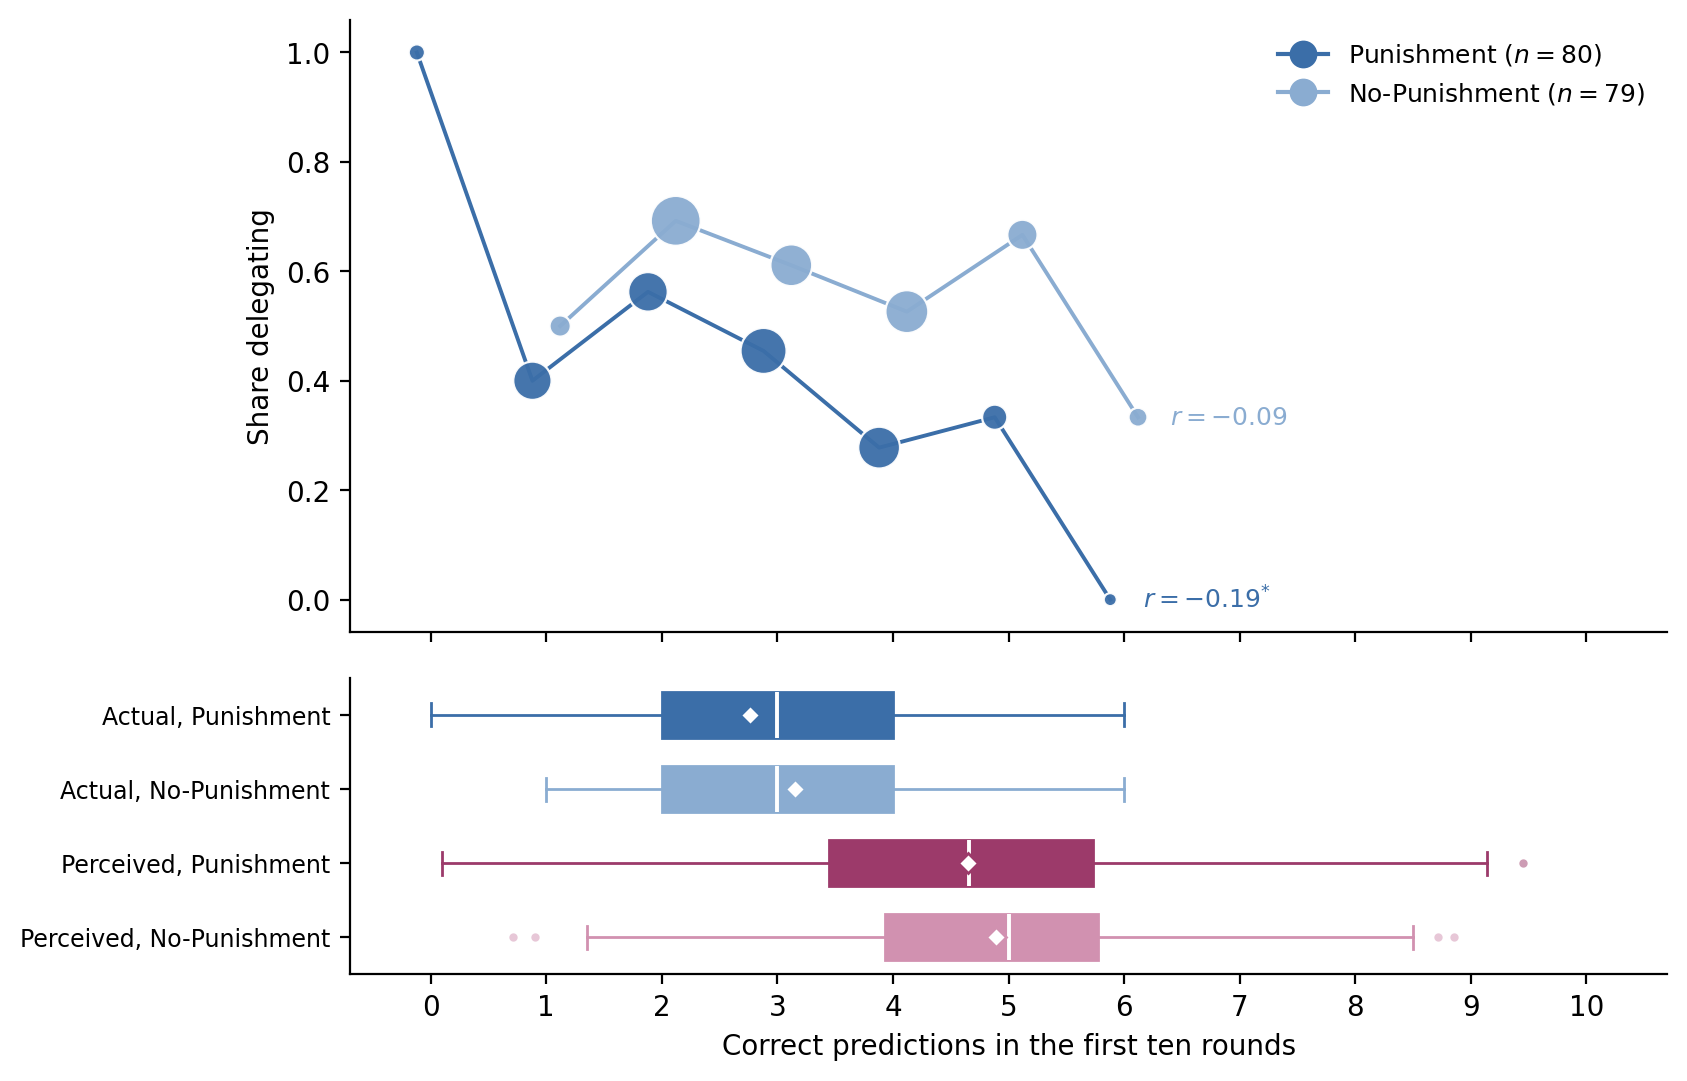
\includegraphics[width=0.9\linewidth]{../quality_reports/exhibits_excl_incredible_guessers/figures/performance_overview.png}
    \label{fig:excl_performance_overview}
\end{figure}

\clearpage

\clearpage
\subsection*{Appendix}

%% ---------------------------------------------------
%% balance_player_a  [CHANGED]   live location: appendix.tex:9
%% ---------------------------------------------------
\begin{table}[!htbp]
    \centering
    \caption{Condition balance --- Player~A}
    \label{tab:excl_treatment_balance}
    \begin{tabular}{l|rrr}
                  Variable &  \textit{Punishment} &  \textit{No-Punishment} &  $p$-value \\ \hline
                           Age &  $39.026$ &  $37.886$ &  $0.557$ \\
                        Female &  $0.487$ &  $0.506$ &  $0.936$ \\
         Socio-economic status &  $5.179$ &  $5.329$ &  $0.542$ \\
                   Went to uni &  $0.575$ &  $0.557$ &  $0.945$ \\
              Technology score &  $2.087$ &  $2.266$ &  $0.366$ \\
           Leadership position &  $0.362$ &  $0.329$ &  $0.783$ \\
    \end{tabular}
    \begin{minipage}{0.95\textwidth}\footnotesize
    \textit{Note:} Mean values by condition for Player~A, with $p$-values from two-sided $t$-tests for continuous variables and Chi-squared tests for binary variables. \textit{Socio-economic status} is self-reported on a $1$--$10$ scale. \textit{Went to uni} indicates a university degree. \textit{Technology score} is constructed from weekly device usage, programming skills, cryptocurrency knowledge, technology use at work, and similar items. \textit{Leadership position} indicates self-reported management or supervisory experience.
    \end{minipage}
\end{table}

\clearpage

%% ---------------------------------------------------
%% reg_punishment_extensive  [IDENTICAL to live]   live location: appendix.tex:19
%% ---------------------------------------------------
\begin{table}[!htbp]
\centering
\scriptsize
\caption{Extensive margin of punishment --- probit for $\Pr(\text{punishment}>0)$}
\label{tab:excl_reg_punishment_extensive}
\begin{tabular}{@{\extracolsep{5pt}}lcc}
\\[-1.8ex]\hline
\hline \\[-1.8ex]
& \multicolumn{2}{c}{Dependent variable: \textit{Any punishment}}\\[0.1cm]
& \textit{Full sample} & \textit{Passers} \\
\\[-1.8ex] & (1) & (2) \\
\hline \\[-1.8ex]
 Delegated & $0.002$ & $-0.042$ \\
  & $(0.077)$ & $(0.078)$ \\[0.1cm]
 Bad outcome & $0.556^{***}$ & $0.563^{***}$ \\
  & $(0.139)$ & $(0.153)$ \\[0.1cm]
 Delegated $\times$ Bad outcome & $-0.099$ & $-0.072$ \\
  & $(0.095)$ & $(0.103)$ \\[0.1cm]
 Player B belief about Player A perf. & $-0.083$ & $-0.030$ \\
  & $(0.075)$ & $(0.082)$ \\[0.1cm]
 Age & $-0.006$ & $-0.013$ \\
  & $(0.013)$ & $(0.015)$ \\[0.1cm]
 Female & $0.115$ & $0.230$ \\
  & $(0.272)$ & $(0.291)$ \\[0.1cm]
 Socio-economic status & $0.160$ & $0.140$ \\
  & $(0.126)$ & $(0.129)$ \\[0.1cm]
 Went to uni & $-0.827^{***}$ & $-0.706^{**}$ \\
  & $(0.320)$ & $(0.349)$ \\[0.1cm]
 Technology score & $0.062$ & $-0.023$ \\
  & $(0.118)$ & $(0.131)$ \\[0.1cm]
 Leadership position & $0.062$ & $-0.071$ \\
  & $(0.293)$ & $(0.321)$ \\[0.1cm]
 Constant & $-0.382$ & $-0.182$ \\
  & $(0.807)$ & $(0.864)$ \\[0.1cm]
\hline \\[-1.8ex]
 AME of Delegated (pp) & $-1.8$ & $-2.9$ \\
  & $(p=0.462)$ & $(p=0.285)$ \\
 AME of Bad outcome (pp) & $18.1^{***}$ & $19.4^{***}$ \\
  & $(p<0.001)$ & $(p<0.001)$ \\
 Observations & $320$ & $268$ \\
 Subjects & $80$ & $67$ \\
 Pseudo $R^2$ & $0.096$ & $0.081$ \\
\hline
\hline \\[-1.8ex]
\multicolumn{3}{c}{\begin{minipage}{0.85\textwidth}\footnotesize \textit{Note:} Probit regression of an indicator for non-zero punishment ($1\{\text{punishment}>0\}$) on a delegation indicator, a bad-outcome indicator, their interaction, Player~B's belief about Player~A's performance, and socio-demographic controls; the sample is stacked over the four (delegation, outcome) cells of the strategy method (4 observations per Player~B). Column~(1) uses the full Punishment-condition sample; Column~(2) restricts to attention-check passers. Standard errors clustered at the Player~B level. The \textit{AME} rows report discrete average marginal effects on the probability of imposing any punishment, in percentage points (for Delegated, the change from $0\to1$ with the interaction moved consistently; for Bad outcome, likewise), computed by counterfactual prediction with p-values from a seeded $400$-replication subject-cluster bootstrap. Significance: $^{*}\,p<0.10$; $^{**}\,p<0.05$; $^{***}\,p<0.01$ (two-sided).\end{minipage}}
\end{tabular}
\end{table}

\clearpage

%% ---------------------------------------------------
%% punishment_passers  [IDENTICAL to live]   live location: appendix.tex:56
%% ---------------------------------------------------
\begin{figure}[!htbp]
    \centering
    \caption{Player~B punishment by delegation and outcome scenario, attention-check passers}
    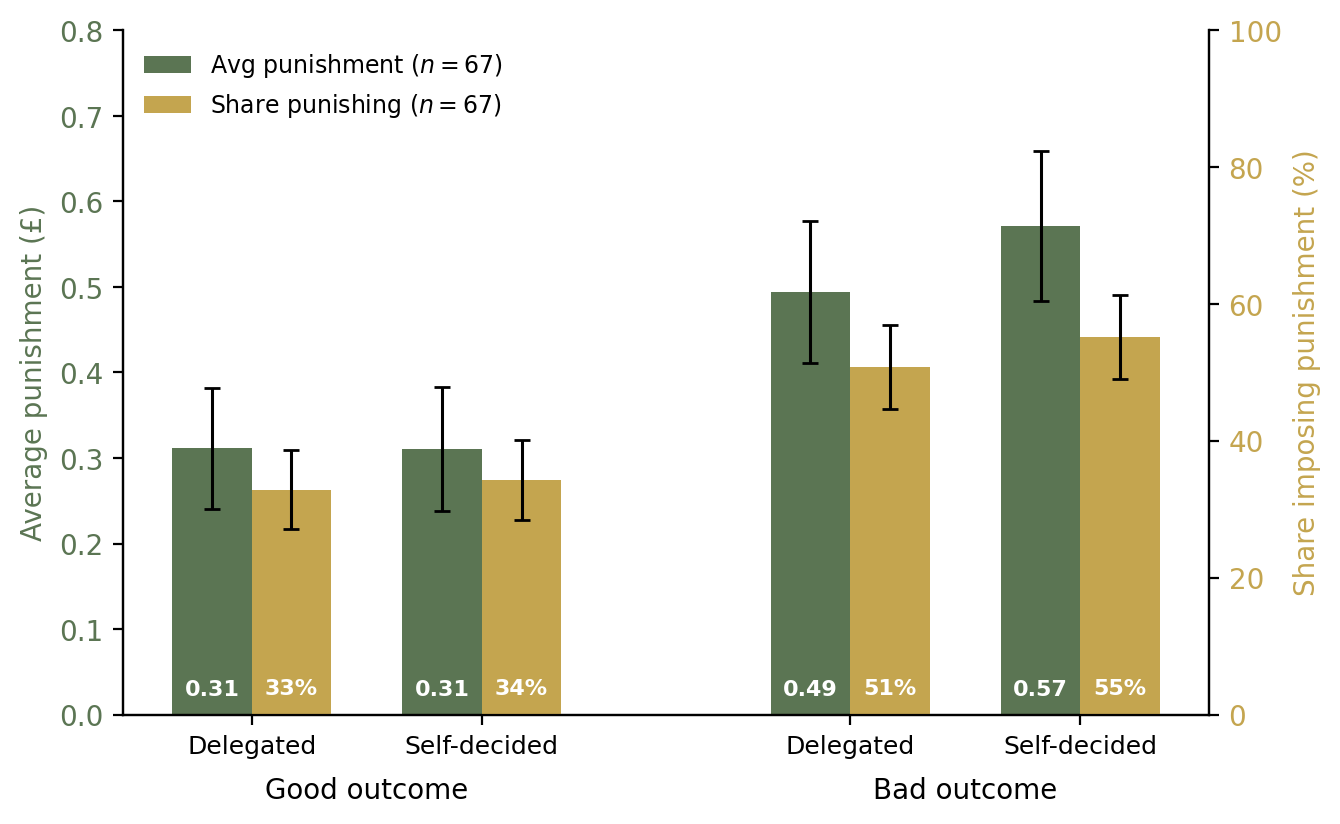
\includegraphics[width=0.65\linewidth]{../quality_reports/exhibits_excl_incredible_guessers/figures/punishment_passers.png}
    \label{fig:excl_punishment_passers}
\end{figure}

\clearpage

%% ---------------------------------------------------
%% realized_vs_anticipated_passers  [IDENTICAL to live]   live location: appendix.tex:67
%% ---------------------------------------------------
\begin{figure}[!htbp]
    \centering
    \caption{Realized vs.\ anticipated punishment, attention-check passers}
    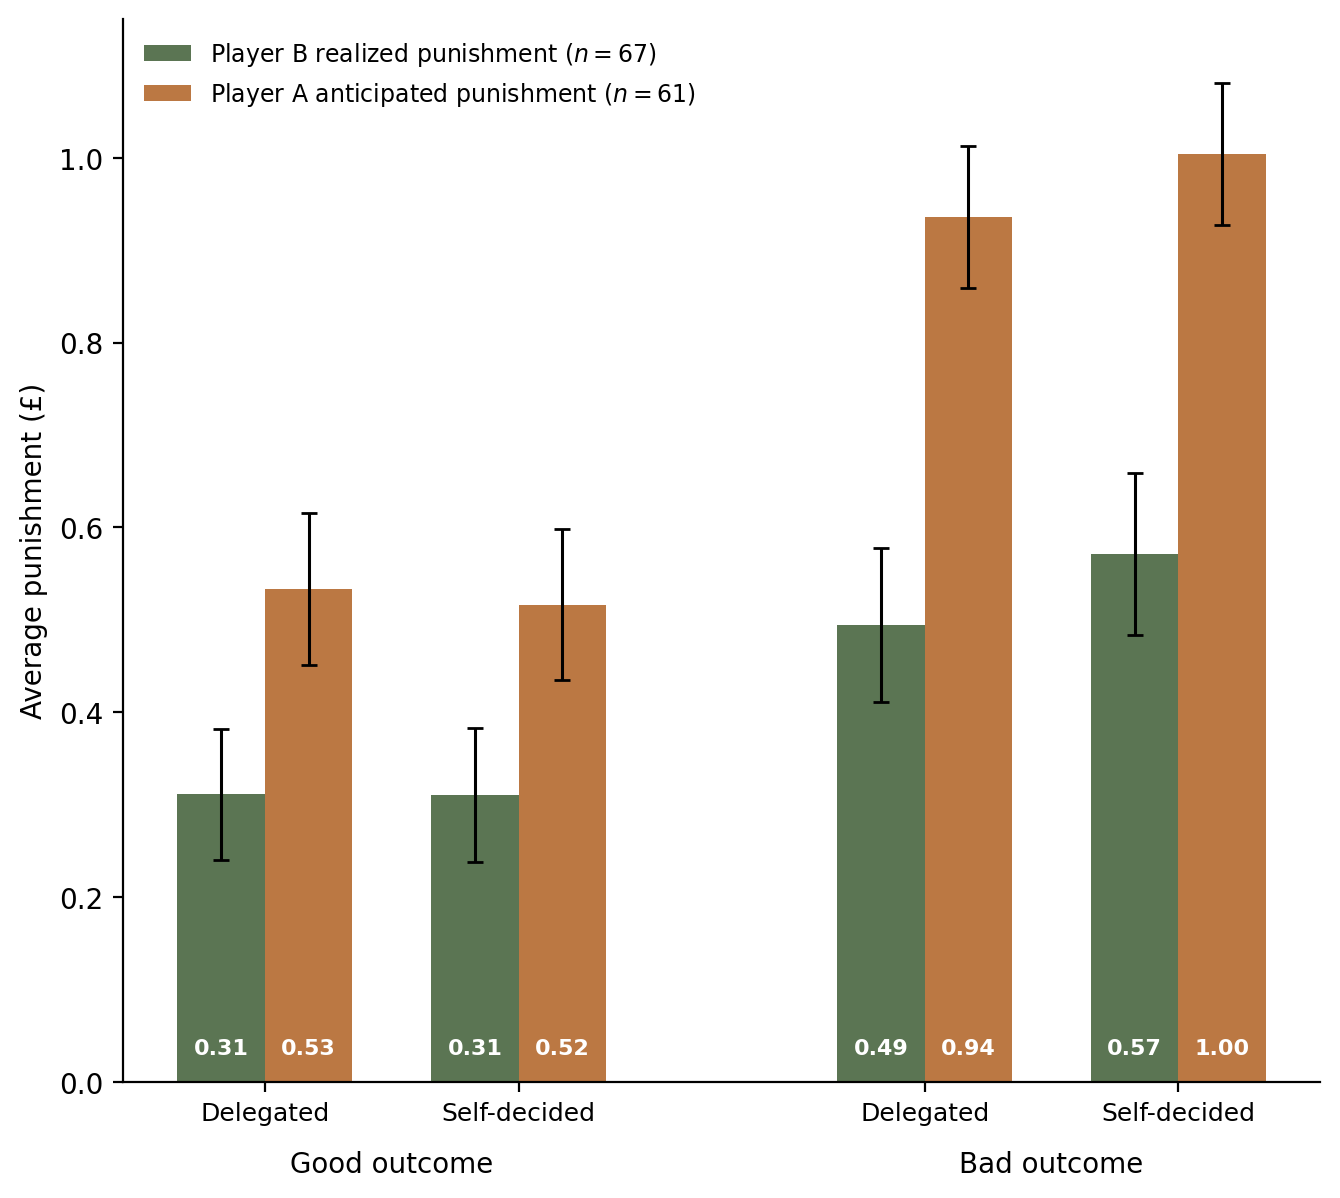
\includegraphics[width=0.75\linewidth]{../quality_reports/exhibits_excl_incredible_guessers/figures/realized_vs_anticipated_passers.png}
    \label{fig:excl_realized_vs_anticipated_passers}
\end{figure}

\clearpage

%% ---------------------------------------------------
%% punishment_hypothetical  [CHANGED]   live location: appendix.tex:83
%% ---------------------------------------------------
\begin{figure}[!htbp]
    \centering
    \caption{Hypothetical punishment by delegation and outcome scenario (\textit{No-Punishment} condition)}
    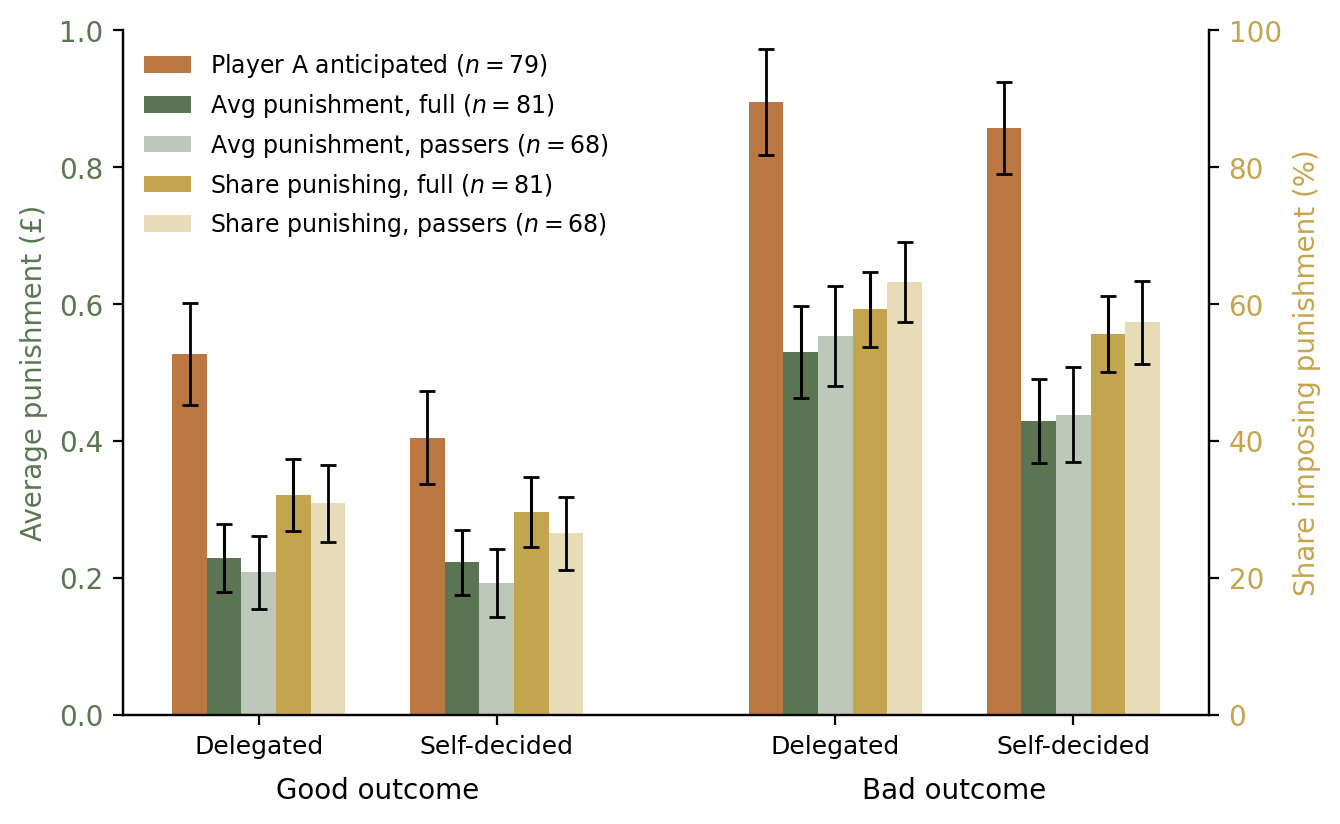
\includegraphics[width=0.65\linewidth]{../quality_reports/exhibits_excl_incredible_guessers/figures/punishment_hypothetical.png}
    \label{fig:excl_punishment_hypothetical}
\end{figure}

\clearpage

%%  from manuscript/main.tex. Every label carries an excl_ prefix, so this
%%  file can coexist with the live exhibits in a single document.
%% =====================================================================

\clearpage
\section*{Exhibits excluding the two incredible weight guessers}

\clearpage
\subsection*{Results}

%% ---------------------------------------------------
%% delegation_shares  [CHANGED]   live location: results.tex:19
%% ---------------------------------------------------
\begin{figure}[!htbp]
    \centering
    \caption{Delegation shares by condition}
    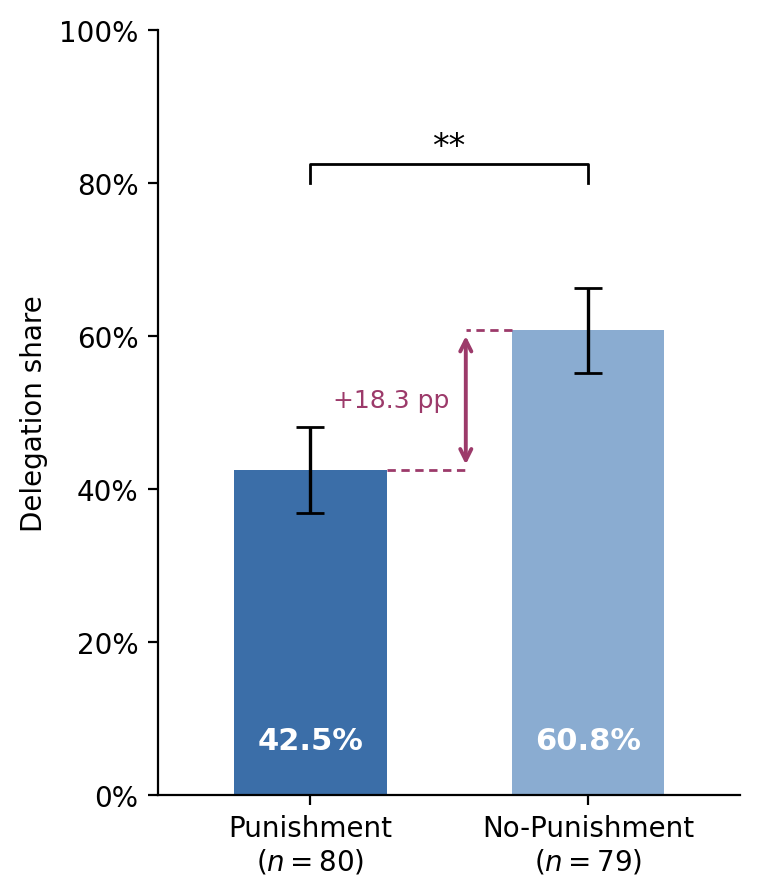
\includegraphics[width=0.5\linewidth]{../quality_reports/exhibits_excl_incredible_guessers/figures/delegation_shares.png}
    \label{fig:excl_delegation_shares}
\end{figure}

\clearpage
%% ---------------------------------------------------
%% reg_delegation  [CHANGED]   live location: results.tex:31
%% ---------------------------------------------------
\begin{table}[!htbp]
\centering
\scriptsize
\caption{Determinants of the delegation decision}
\label{tab:excl_del_decision_determinants}
\begin{tabular}{@{\extracolsep{5pt}}lcccc|c}
\\[-1.8ex]\hline
\hline \\[-1.8ex]
& \multicolumn{5}{c}{Dependent variable: \textit{Delegation}}\\[0.1cm]
& \multicolumn{4}{c}{\textit{Full sample}} & \textit{Passers} \\
\\[-1.8ex] & (1) & (2) & (3) & (4) & (5) \\
\hline \\[-1.8ex]
 Punishment indicator & $-0.462^{**}$ & $-0.473^{**}$ & $-0.537^{**}$ & $-0.489^{**}$ & $-0.589^{**}$ \\
  & $(0.201)$ & $(0.206)$ & $(0.209)$ & $(0.207)$ & $(0.235)$ \\[0.1cm]
 Task performance &  &  & $-0.160^{**}$ &  & $-0.203^{**}$ \\
  &  &  & $(0.081)$ &  & $(0.089)$ \\[0.1cm]
 Perceived performance &  &  &  & $-0.075$ &  \\
  &  &  &  & $(0.057)$ &  \\[0.1cm]
 Age &  & $-0.003$ & $-0.002$ & $-0.002$ & $0.002$ \\
  &  & $(0.009)$ & $(0.009)$ & $(0.009)$ & $(0.011)$ \\[0.1cm]
 Female &  & $0.141$ & $0.194$ & $0.181$ & $0.372$ \\
  &  & $(0.228)$ & $(0.230)$ & $(0.231)$ & $(0.257)$ \\[0.1cm]
 Socio-economic status &  & $-0.044$ & $-0.042$ & $-0.036$ & $-0.086$ \\
  &  & $(0.071)$ & $(0.073)$ & $(0.072)$ & $(0.081)$ \\[0.1cm]
 Went to uni &  & $0.032$ & $0.062$ & $0.020$ & $0.118$ \\
  &  & $(0.228)$ & $(0.226)$ & $(0.227)$ & $(0.248)$ \\[0.1cm]
 Technology score &  & $-0.065$ & $-0.036$ & $-0.056$ & $0.024$ \\
  &  & $(0.093)$ & $(0.096)$ & $(0.093)$ & $(0.109)$ \\[0.1cm]
 Leadership position &  & $0.415^{*}$ & $0.444^{*}$ & $0.411^{*}$ & $0.278$ \\
  &  & $(0.226)$ & $(0.228)$ & $(0.226)$ & $(0.256)$ \\[0.1cm]
 Constant & $0.273^{*}$ & $0.533$ & $0.908$ & $0.801$ & $0.851$ \\
  & $(0.143)$ & $(0.557)$ & $(0.593)$ & $(0.606)$ & $(0.673)$ \\[0.1cm]
\hline \\[-1.8ex]
 AME of Punishment (pp) & $-18.3^{**}$ & $-18.3^{**}$ & $-20.3^{***}$ & $-18.7^{**}$ & $-21.8^{***}$ \\
  & $(p=0.019)$ & $(p=0.019)$ & $(p=0.008)$ & $(p=0.016)$ & $(p=0.009)$ \\
 N & $159$ & $157$ & $157$ & $157$ & $128$ \\
 Pseudo $R^2$ & $0.024$ & $0.042$ & $0.060$ & $0.051$ & $0.077$ \\
\hline
\hline \\[-1.8ex]
\multicolumn{6}{c}{\begin{minipage}{0.85\textwidth}\footnotesize \textit{Note:} Coefficients from a Probit regression of the delegation decision on the Punishment indicator and a set of controls. Robust (HC1) standard errors in parentheses. Significance: $^{*}\,p<0.10$; $^{**}\,p<0.05$; $^{***}\,p<0.01$ (two-sided). Due to missing socio-demographic data, two subjects are dropped in Columns~(2)--(5). The \textit{AME of Punishment} reports the average change in the predicted probability of delegation from introducing the punishment possibility, in percentage points.\end{minipage}}
\end{tabular}
\end{table}

\clearpage

%% ---------------------------------------------------
%% punishment  [IDENTICAL to live]   live location: results.tex:40
%% ---------------------------------------------------
\begin{figure}[!htbp]
    \centering
    \caption{Player~B punishment by delegation and outcome scenario}
    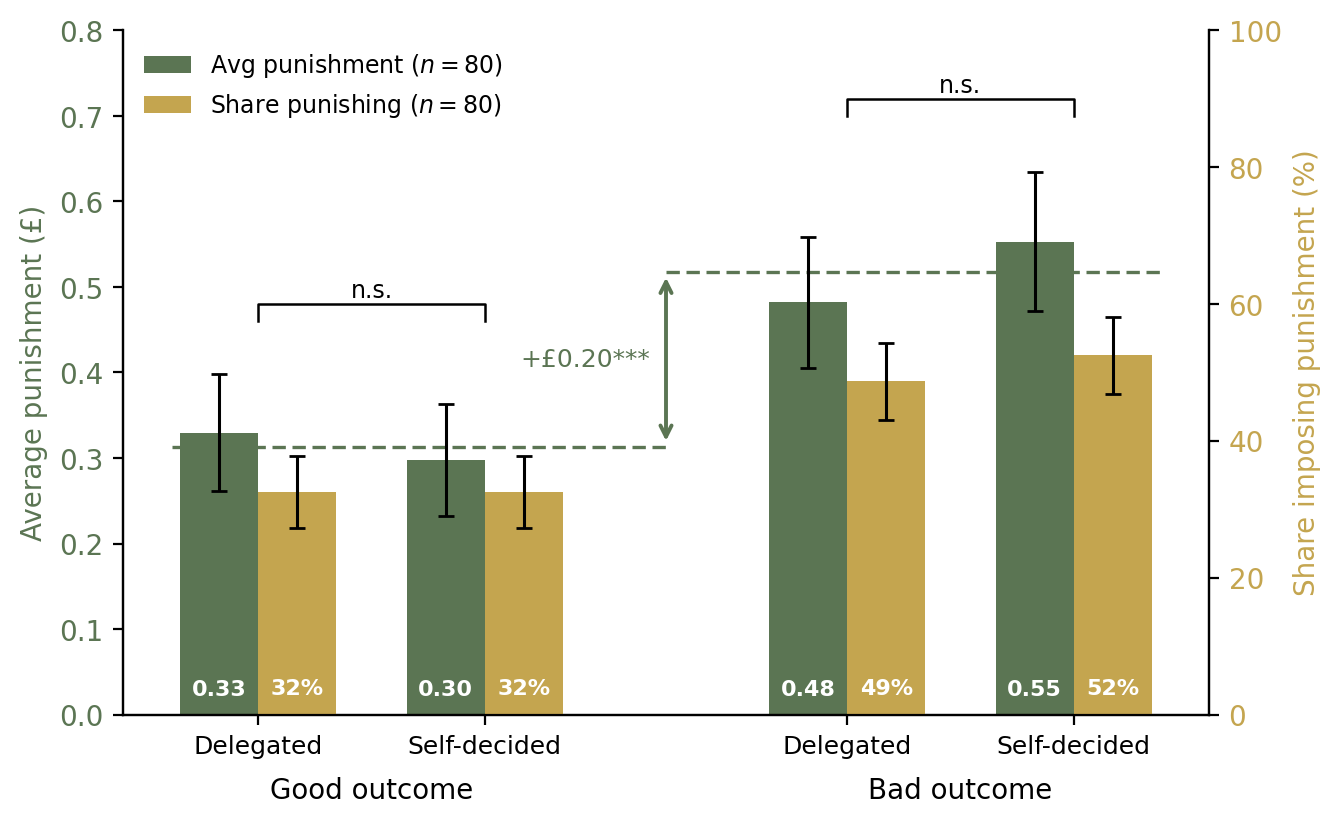
\includegraphics[width=0.75\linewidth]{../quality_reports/exhibits_excl_incredible_guessers/figures/punishment.png}
    \label{fig:excl_punishment}
\end{figure}

\clearpage
%% ---------------------------------------------------
%% reg_punishment  [IDENTICAL to live]   live location: results.tex:58
%% ---------------------------------------------------
\begin{table}[!htbp]
\centering
\scriptsize
\caption{Determinants of Player~B's chosen punishment}
\label{tab:excl_reg_punishment}
\begin{tabular}{@{\extracolsep{5pt}}lcc}
\\[-1.8ex]\hline
\hline \\[-1.8ex]
& \multicolumn{2}{c}{Dependent variable: \textit{Punishment (\pounds)}}\\[0.1cm]
& \textit{Full sample} & \textit{Passers} \\
\\[-1.8ex] & (1) & (2) \\
\hline \\[-1.8ex]
 Delegated & $0.032$ & $0.001$ \\
  & $(0.052)$ & $(0.054)$ \\[0.1cm]
 Bad outcome & $0.256^{***}$ & $0.260^{***}$ \\
  & $(0.071)$ & $(0.080)$ \\[0.1cm]
 Delegated $\times$ Bad outcome & $-0.103^{*}$ & $-0.078$ \\
  & $(0.058)$ & $(0.052)$ \\[0.1cm]
 Player B belief about Player A perf. & $-0.020$ & $0.001$ \\
  & $(0.032)$ & $(0.037)$ \\[0.1cm]
 Age & $0.002$ & $-0.001$ \\
  & $(0.005)$ & $(0.006)$ \\[0.1cm]
 Female & $-0.100$ & $-0.064$ \\
  & $(0.128)$ & $(0.140)$ \\[0.1cm]
 Socio-economic status & $0.083^{*}$ & $0.072$ \\
  & $(0.047)$ & $(0.049)$ \\[0.1cm]
 Went to uni & $-0.196$ & $-0.098$ \\
  & $(0.140)$ & $(0.142)$ \\[0.1cm]
 Technology score & $0.073$ & $0.030$ \\
  & $(0.053)$ & $(0.059)$ \\[0.1cm]
 Leadership position & $0.083$ & $0.061$ \\
  & $(0.142)$ & $(0.164)$ \\[0.1cm]
 Constant & $-0.077$ & $0.020$ \\
  & $(0.328)$ & $(0.374)$ \\[0.1cm]
\hline \\[-1.8ex]
 Observations & $320$ & $268$ \\
 Subjects & $80$ & $67$ \\
 Adj.\ $R^2$ & $0.077$ & $0.030$ \\
\hline
\hline \\[-1.8ex]
\multicolumn{3}{c}{\begin{minipage}{0.75\textwidth}\footnotesize \textit{Note:} OLS regression of Player~B's chosen punishment levels. The sample is stacked over the four (delegation, outcome) scenarios of the strategy method (4 observations per Player~B). Column~(1) uses the full Punishment-condition sample. Column~(2) restricts to Player~Bs who passed the attention check on the punishment-elicitation screen. Standard errors clustered at the Player~B level.\end{minipage}}
\end{tabular}
\end{table}

\clearpage

%% ---------------------------------------------------
%% realized_vs_anticipated  [IDENTICAL to live]   live location: results.tex:86
%% ---------------------------------------------------
\begin{figure}[!htbp]
    \centering
    \caption{Realized vs.\ anticipated punishment, by scenario}
    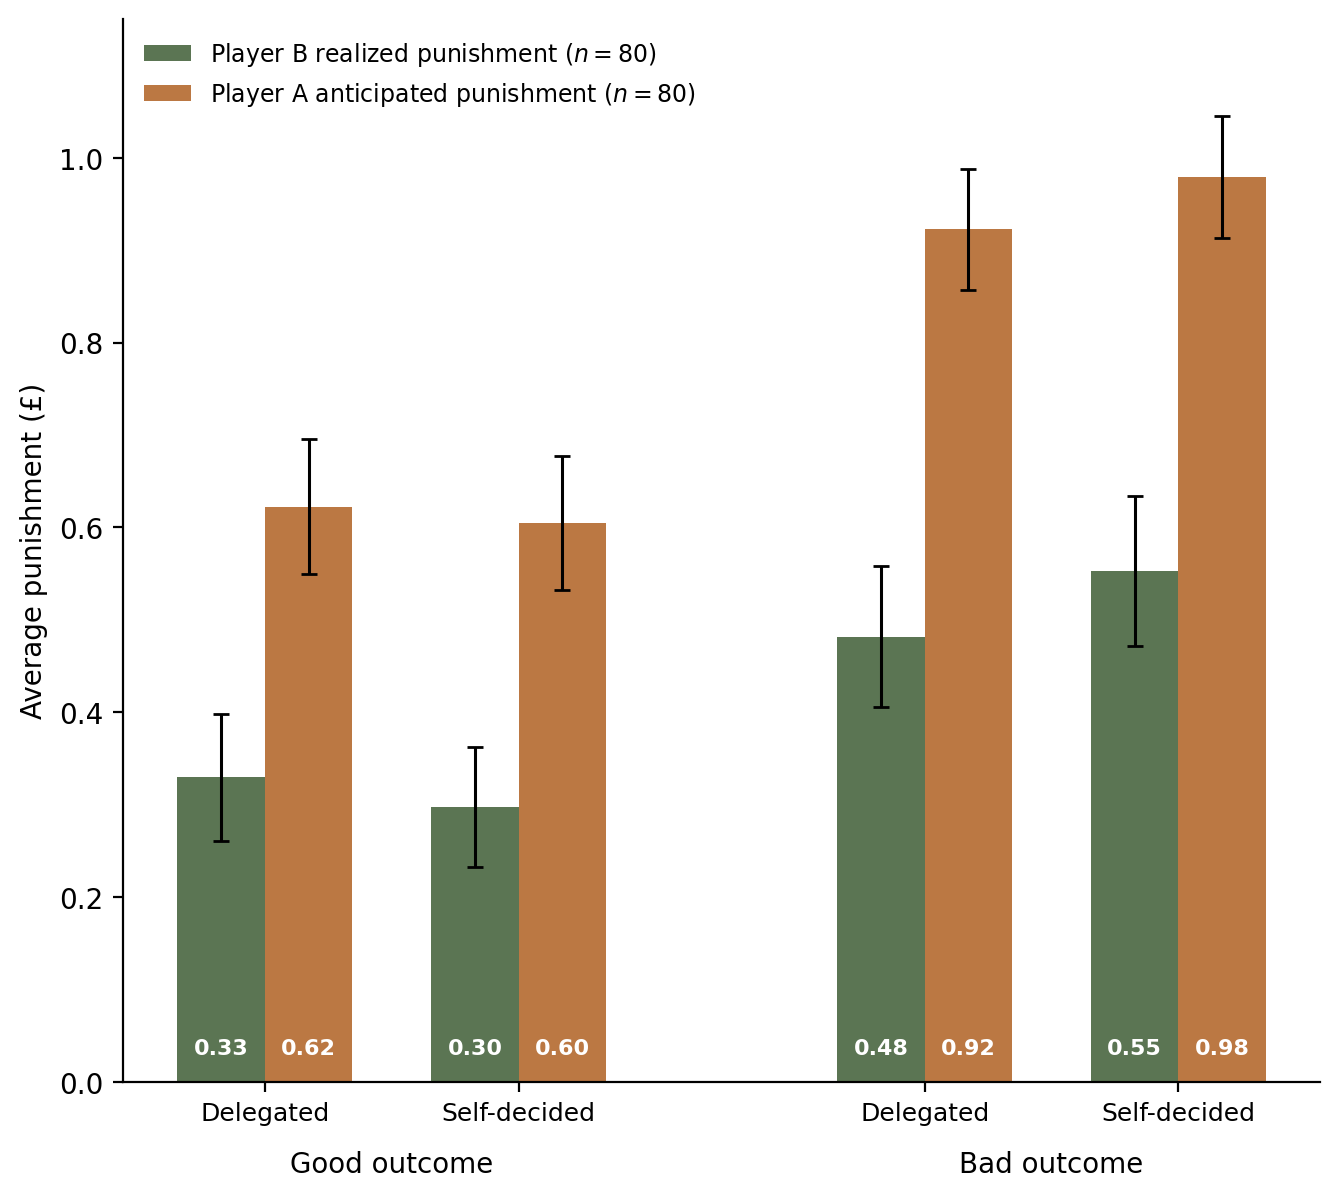
\includegraphics[width=0.75\linewidth]{../quality_reports/exhibits_excl_incredible_guessers/figures/realized_vs_anticipated.png}
    \label{fig:excl_realized_vs_anticipated}
\end{figure}

\clearpage

%% ---------------------------------------------------
%% reg_belief_specs  [IDENTICAL to live]   live location: results.tex:98
%% ---------------------------------------------------
\begin{table}[!htbp]
\centering
\scriptsize
\caption{Delegation and beliefs about punishment}
\label{tab:excl_reg_belief_specs}
\begin{tabular}{@{\extracolsep{5pt}}lcc|ccc}
\\[-1.8ex]\hline
\hline \\[-1.8ex]
& \multicolumn{5}{c}{Dependent variable: \textit{Delegation}}\\[0.1cm]
& \multicolumn{2}{c}{\textit{Full Punishment}} & \multicolumn{3}{c}{\textit{Punishment, passers}} \\
\\[-1.8ex] & (1) & (2) & (3) & (4) & (5) \\
\hline \\[-1.8ex]
 Belief difference, average ($\overline{\Delta}$) & $0.346$ & $0.398$ & $1.661^{**}$ &  &  \\
  & $(0.407)$ & $(0.448)$ & $(0.700)$ &  &  \\[0.1cm]
 Belief difference, weighted by $\Pr(\text{good})$ ($\Delta^{w}$) &  &  &  & $1.992^{**}$ &  \\
  &  &  &  & $(0.794)$ &  \\[0.1cm]
 Belief difference, bad outcome ($\Delta^{\text{bad}}$) &  &  &  &  & $0.590$ \\
  &  &  &  &  & $(0.424)$ \\[0.1cm]
 Belief difference, good outcome ($\Delta^{\text{good}}$) &  &  &  &  & $0.961^{**}$ \\
  &  &  &  &  & $(0.412)$ \\[0.1cm]
 Task performance &  & $-0.208^{*}$ & $-0.362^{***}$ & $-0.342^{**}$ & $-0.381^{***}$ \\
  &  & $(0.111)$ & $(0.136)$ & $(0.142)$ & $(0.138)$ \\[0.1cm]
 Age &  & $0.023^{*}$ & $0.039^{**}$ & $0.040^{**}$ & $0.039^{**}$ \\
  &  & $(0.012)$ & $(0.016)$ & $(0.016)$ & $(0.016)$ \\[0.1cm]
 Female &  & $0.152$ & $0.950^{**}$ & $1.026^{**}$ & $0.845^{*}$ \\
  &  & $(0.350)$ & $(0.427)$ & $(0.406)$ & $(0.444)$ \\[0.1cm]
 Socio-economic status &  & $-0.049$ & $-0.006$ & $-0.055$ & $0.001$ \\
  &  & $(0.111)$ & $(0.131)$ & $(0.133)$ & $(0.126)$ \\[0.1cm]
 Went to uni &  & $0.071$ & $-0.278$ & $-0.169$ & $-0.275$ \\
  &  & $(0.363)$ & $(0.412)$ & $(0.408)$ & $(0.409)$ \\[0.1cm]
 Technology score &  & $-0.061$ & $0.048$ & $0.072$ & $0.033$ \\
  &  & $(0.138)$ & $(0.170)$ & $(0.173)$ & $(0.167)$ \\[0.1cm]
 Leadership position &  & $0.302$ & $-0.301$ & $-0.279$ & $-0.245$ \\
  &  & $(0.312)$ & $(0.408)$ & $(0.408)$ & $(0.411)$ \\[0.1cm]
 Constant & $-0.198$ & $-0.345$ & $-1.228$ & $-1.281$ & $-1.115$ \\
  & $(0.142)$ & $(0.826)$ & $(1.155)$ & $(1.147)$ & $(1.165)$ \\[0.1cm]
\hline \\[-1.8ex]
 AME of belief measure (pp per \pounds 0.10) & $1.3$ & $1.4$ & $4.7^{**}$ & $5.5^{***}$ &  \\
  & $(p=0.388)$ & $(p=0.370)$ & $(p=0.011)$ & $(p=0.006)$ &  \\
 AME: good-outcome difference (pp per \pounds 0.10) &  &  &  &  & $2.7^{**}$ \\
  &  &  &  &  & $(p=0.010)$ \\
 AME: bad-outcome difference (pp per \pounds 0.10) &  &  &  &  & $1.7$ \\
  &  &  &  &  & $(p=0.165)$ \\
 Controls & $\times$ & \checkmark & \checkmark & \checkmark & \checkmark \\
 Passers only & $\times$ & $\times$ & \checkmark & \checkmark & \checkmark \\
 N & $80$ & $78$ & $60$ & $60$ & $60$ \\
 Pseudo $R^2$ & $0.007$ & $0.098$ & $0.248$ & $0.263$ & $0.252$ \\
\hline
\hline \\[-1.8ex]
\multicolumn{6}{c}{\begin{minipage}{0.92\textwidth}\footnotesize \textit{Note:} Probit estimates with robust (HC1) standard errors in parentheses. Sample restricted to the \textit{Punishment} condition throughout. Belief differences are within-subject \textit{(no delegation)}~$-$~\textit{(delegation)} in expected punishment, so positive coefficients indicate that subjects who expect to be punished more harshly for not delegating (relative to delegating) are more likely to delegate. Columns~(1)--(3) use the simple average of the good-outcome and the bad-outcome belief difference. Column~(4) instead weights the good-outcome difference by Player~A's elicited probability of producing the high payoff and the bad-outcome difference by the complementary probability. Column~(5) enters the two differences separately. The \textit{AME} rows report the average marginal effect of the belief measure entered in the respective column on the probability of delegation, in percentage points per \pounds 0.10 increase in the corresponding belief difference.\end{minipage}}
\end{tabular}
\end{table}

\clearpage

%% ---------------------------------------------------
%% performance_overview  [CHANGED]   live location: results.tex:121
%% ---------------------------------------------------
\begin{figure}[!htbp]
    \centering
    \caption{Delegation, performance, and confidence by condition}
    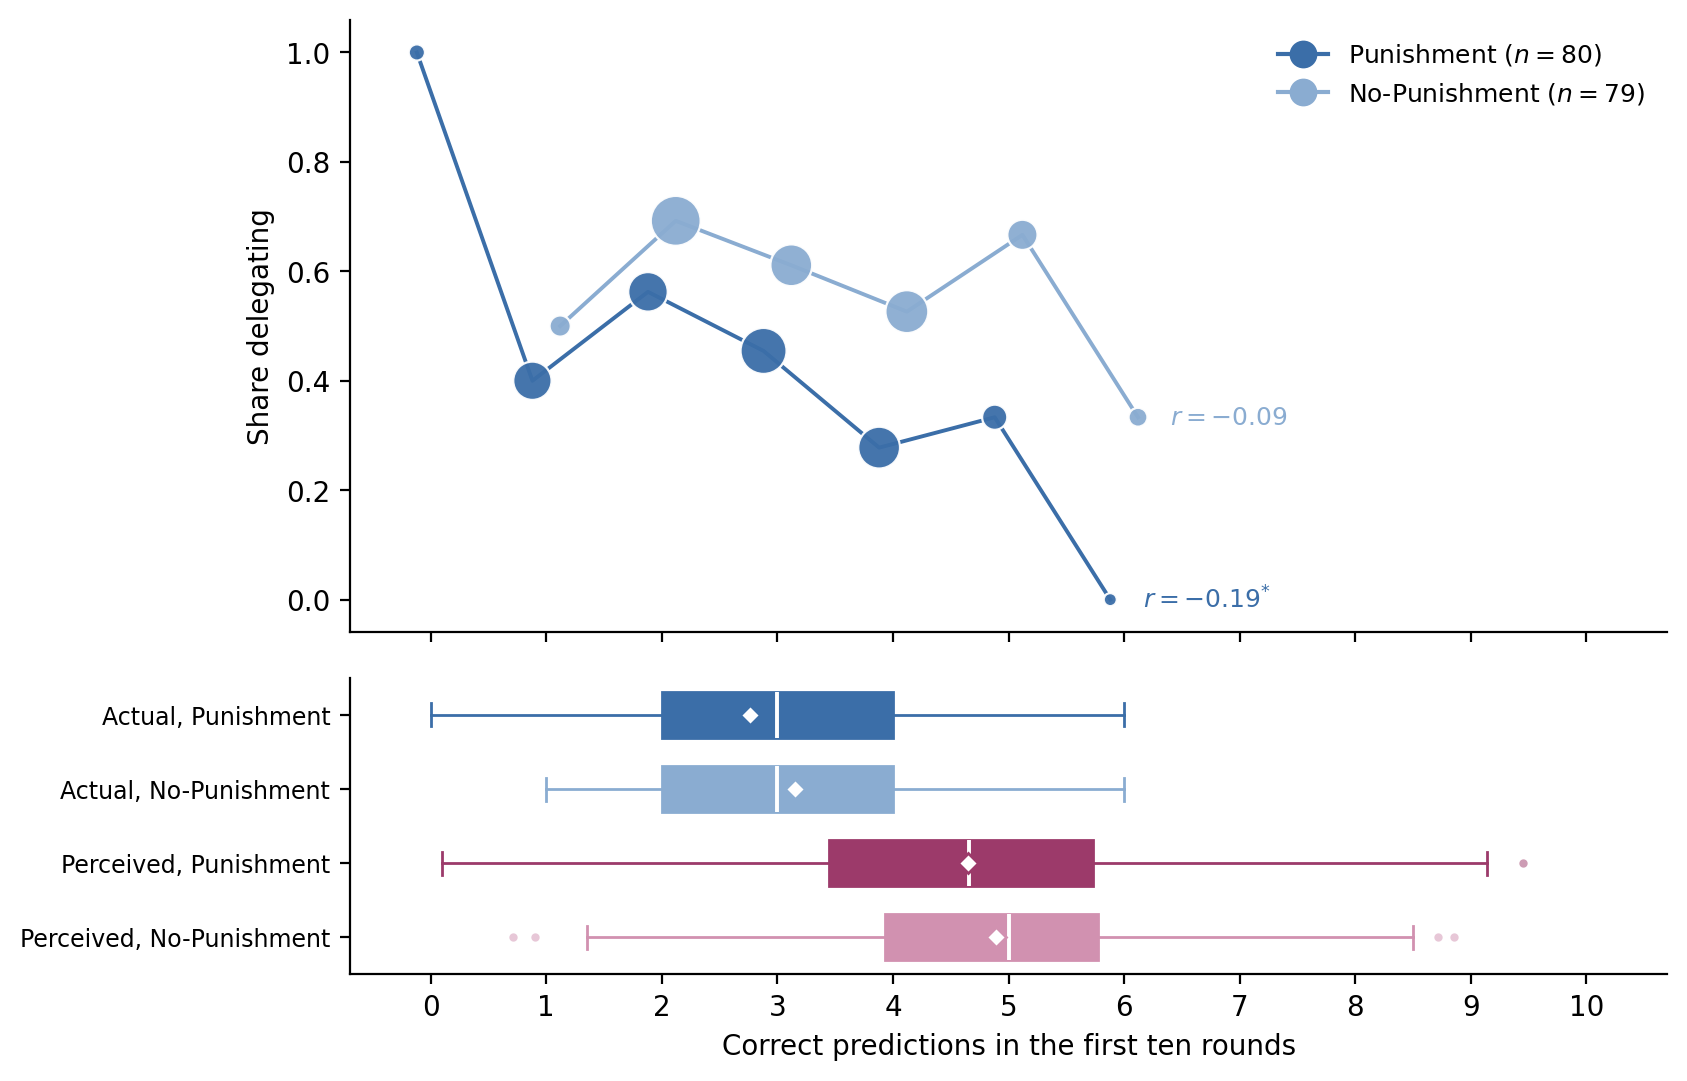
\includegraphics[width=0.9\linewidth]{../quality_reports/exhibits_excl_incredible_guessers/figures/performance_overview.png}
    \label{fig:excl_performance_overview}
\end{figure}

\clearpage

\clearpage
\subsection*{Appendix}

%% ---------------------------------------------------
%% balance_player_a  [CHANGED]   live location: appendix.tex:9
%% ---------------------------------------------------
\begin{table}[!htbp]
    \centering
    \caption{Condition balance --- Player~A}
    \label{tab:excl_treatment_balance}
    \begin{tabular}{l|rrr}
                  Variable &  \textit{Punishment} &  \textit{No-Punishment} &  $p$-value \\ \hline
                           Age &  $39.026$ &  $37.886$ &  $0.557$ \\
                        Female &  $0.487$ &  $0.506$ &  $0.936$ \\
         Socio-economic status &  $5.179$ &  $5.329$ &  $0.542$ \\
                   Went to uni &  $0.575$ &  $0.557$ &  $0.945$ \\
              Technology score &  $2.087$ &  $2.266$ &  $0.366$ \\
           Leadership position &  $0.362$ &  $0.329$ &  $0.783$ \\
    \end{tabular}
    \begin{minipage}{0.95\textwidth}\footnotesize
    \textit{Note:} Mean values by condition for Player~A, with $p$-values from two-sided $t$-tests for continuous variables and Chi-squared tests for binary variables. \textit{Socio-economic status} is self-reported on a $1$--$10$ scale. \textit{Went to uni} indicates a university degree. \textit{Technology score} is constructed from weekly device usage, programming skills, cryptocurrency knowledge, technology use at work, and similar items. \textit{Leadership position} indicates self-reported management or supervisory experience.
    \end{minipage}
\end{table}

\clearpage

%% ---------------------------------------------------
%% reg_punishment_extensive  [IDENTICAL to live]   live location: appendix.tex:19
%% ---------------------------------------------------
\begin{table}[!htbp]
\centering
\scriptsize
\caption{Extensive margin of punishment --- probit for $\Pr(\text{punishment}>0)$}
\label{tab:excl_reg_punishment_extensive}
\begin{tabular}{@{\extracolsep{5pt}}lcc}
\\[-1.8ex]\hline
\hline \\[-1.8ex]
& \multicolumn{2}{c}{Dependent variable: \textit{Any punishment}}\\[0.1cm]
& \textit{Full sample} & \textit{Passers} \\
\\[-1.8ex] & (1) & (2) \\
\hline \\[-1.8ex]
 Delegated & $0.002$ & $-0.042$ \\
  & $(0.077)$ & $(0.078)$ \\[0.1cm]
 Bad outcome & $0.556^{***}$ & $0.563^{***}$ \\
  & $(0.139)$ & $(0.153)$ \\[0.1cm]
 Delegated $\times$ Bad outcome & $-0.099$ & $-0.072$ \\
  & $(0.095)$ & $(0.103)$ \\[0.1cm]
 Player B belief about Player A perf. & $-0.083$ & $-0.030$ \\
  & $(0.075)$ & $(0.082)$ \\[0.1cm]
 Age & $-0.006$ & $-0.013$ \\
  & $(0.013)$ & $(0.015)$ \\[0.1cm]
 Female & $0.115$ & $0.230$ \\
  & $(0.272)$ & $(0.291)$ \\[0.1cm]
 Socio-economic status & $0.160$ & $0.140$ \\
  & $(0.126)$ & $(0.129)$ \\[0.1cm]
 Went to uni & $-0.827^{***}$ & $-0.706^{**}$ \\
  & $(0.320)$ & $(0.349)$ \\[0.1cm]
 Technology score & $0.062$ & $-0.023$ \\
  & $(0.118)$ & $(0.131)$ \\[0.1cm]
 Leadership position & $0.062$ & $-0.071$ \\
  & $(0.293)$ & $(0.321)$ \\[0.1cm]
 Constant & $-0.382$ & $-0.182$ \\
  & $(0.807)$ & $(0.864)$ \\[0.1cm]
\hline \\[-1.8ex]
 AME of Delegated (pp) & $-1.8$ & $-2.9$ \\
  & $(p=0.462)$ & $(p=0.285)$ \\
 AME of Bad outcome (pp) & $18.1^{***}$ & $19.4^{***}$ \\
  & $(p<0.001)$ & $(p<0.001)$ \\
 Observations & $320$ & $268$ \\
 Subjects & $80$ & $67$ \\
 Pseudo $R^2$ & $0.096$ & $0.081$ \\
\hline
\hline \\[-1.8ex]
\multicolumn{3}{c}{\begin{minipage}{0.85\textwidth}\footnotesize \textit{Note:} Probit regression of an indicator for non-zero punishment ($1\{\text{punishment}>0\}$) on a delegation indicator, a bad-outcome indicator, their interaction, Player~B's belief about Player~A's performance, and socio-demographic controls; the sample is stacked over the four (delegation, outcome) cells of the strategy method (4 observations per Player~B). Column~(1) uses the full Punishment-condition sample; Column~(2) restricts to attention-check passers. Standard errors clustered at the Player~B level. The \textit{AME} rows report discrete average marginal effects on the probability of imposing any punishment, in percentage points (for Delegated, the change from $0\to1$ with the interaction moved consistently; for Bad outcome, likewise), computed by counterfactual prediction with p-values from a seeded $400$-replication subject-cluster bootstrap. Significance: $^{*}\,p<0.10$; $^{**}\,p<0.05$; $^{***}\,p<0.01$ (two-sided).\end{minipage}}
\end{tabular}
\end{table}

\clearpage

%% ---------------------------------------------------
%% punishment_passers  [IDENTICAL to live]   live location: appendix.tex:56
%% ---------------------------------------------------
\begin{figure}[!htbp]
    \centering
    \caption{Player~B punishment by delegation and outcome scenario, attention-check passers}
    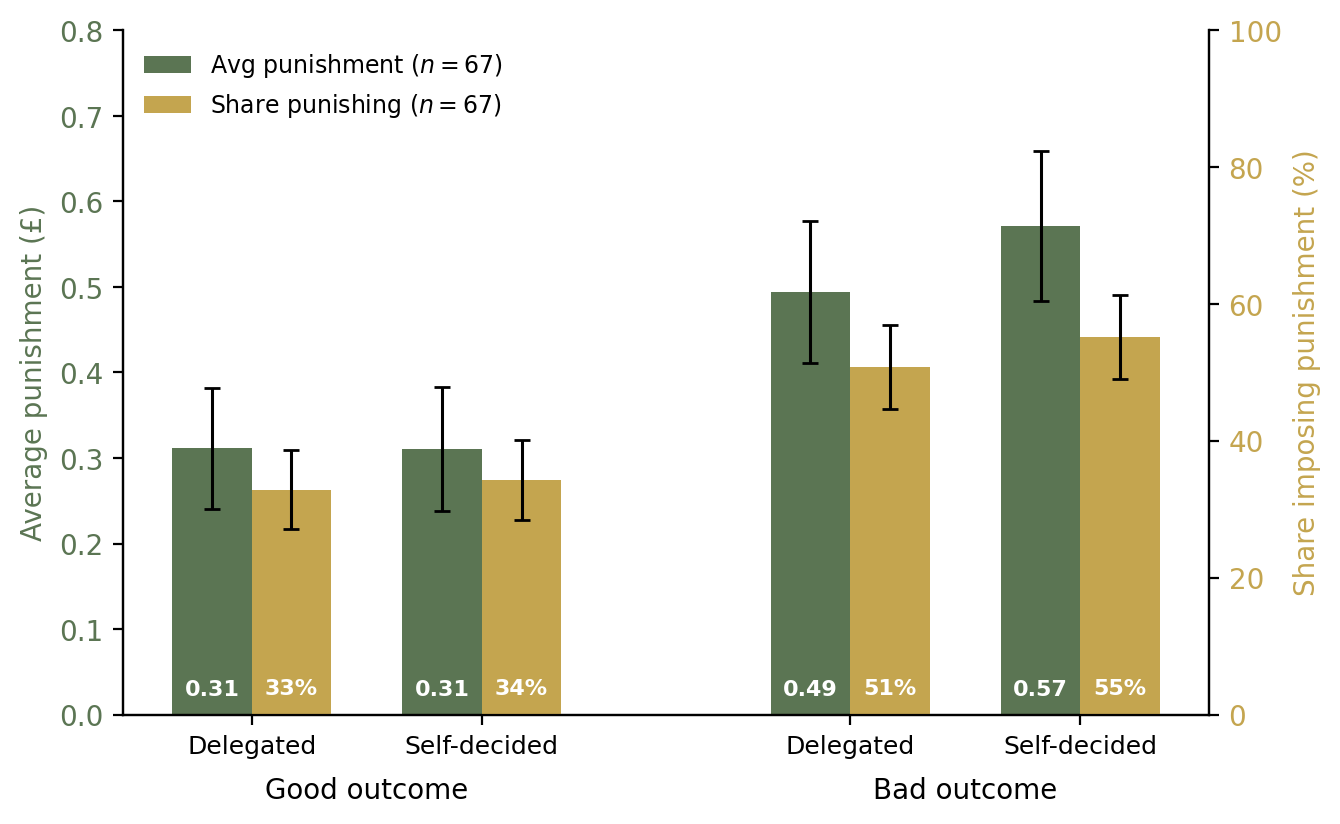
\includegraphics[width=0.65\linewidth]{../quality_reports/exhibits_excl_incredible_guessers/figures/punishment_passers.png}
    \label{fig:excl_punishment_passers}
\end{figure}

\clearpage

%% ---------------------------------------------------
%% realized_vs_anticipated_passers  [IDENTICAL to live]   live location: appendix.tex:67
%% ---------------------------------------------------
\begin{figure}[!htbp]
    \centering
    \caption{Realized vs.\ anticipated punishment, attention-check passers}
    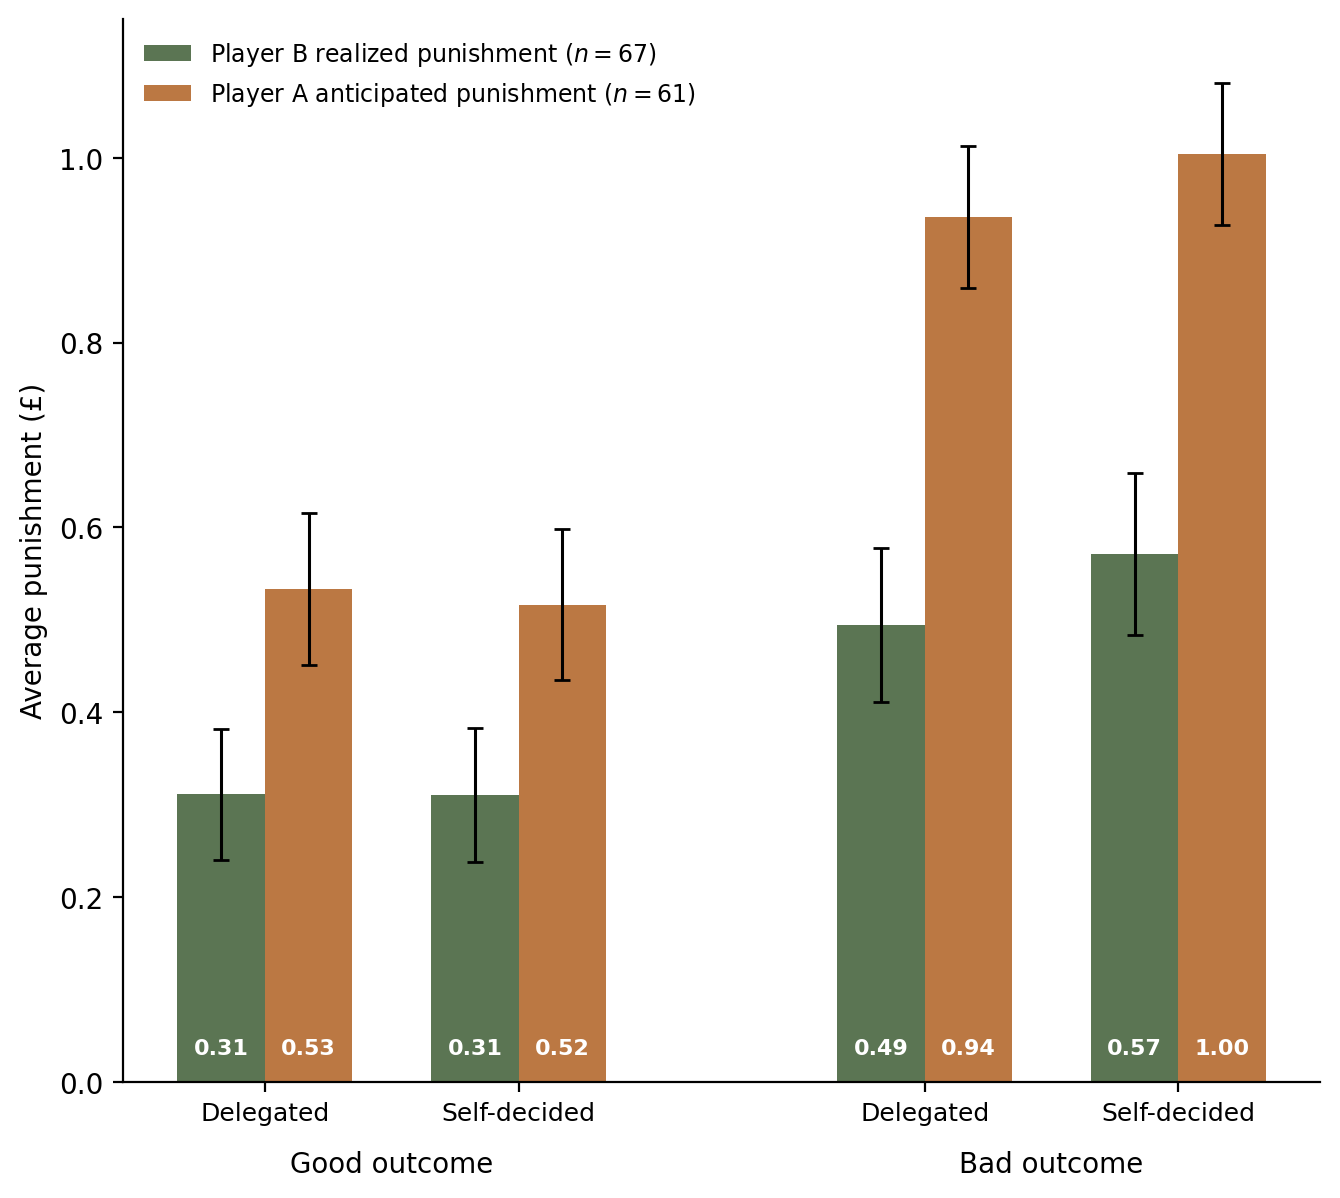
\includegraphics[width=0.75\linewidth]{../quality_reports/exhibits_excl_incredible_guessers/figures/realized_vs_anticipated_passers.png}
    \label{fig:excl_realized_vs_anticipated_passers}
\end{figure}

\clearpage

%% ---------------------------------------------------
%% punishment_hypothetical  [CHANGED]   live location: appendix.tex:83
%% ---------------------------------------------------
\begin{figure}[!htbp]
    \centering
    \caption{Hypothetical punishment by delegation and outcome scenario (\textit{No-Punishment} condition)}
    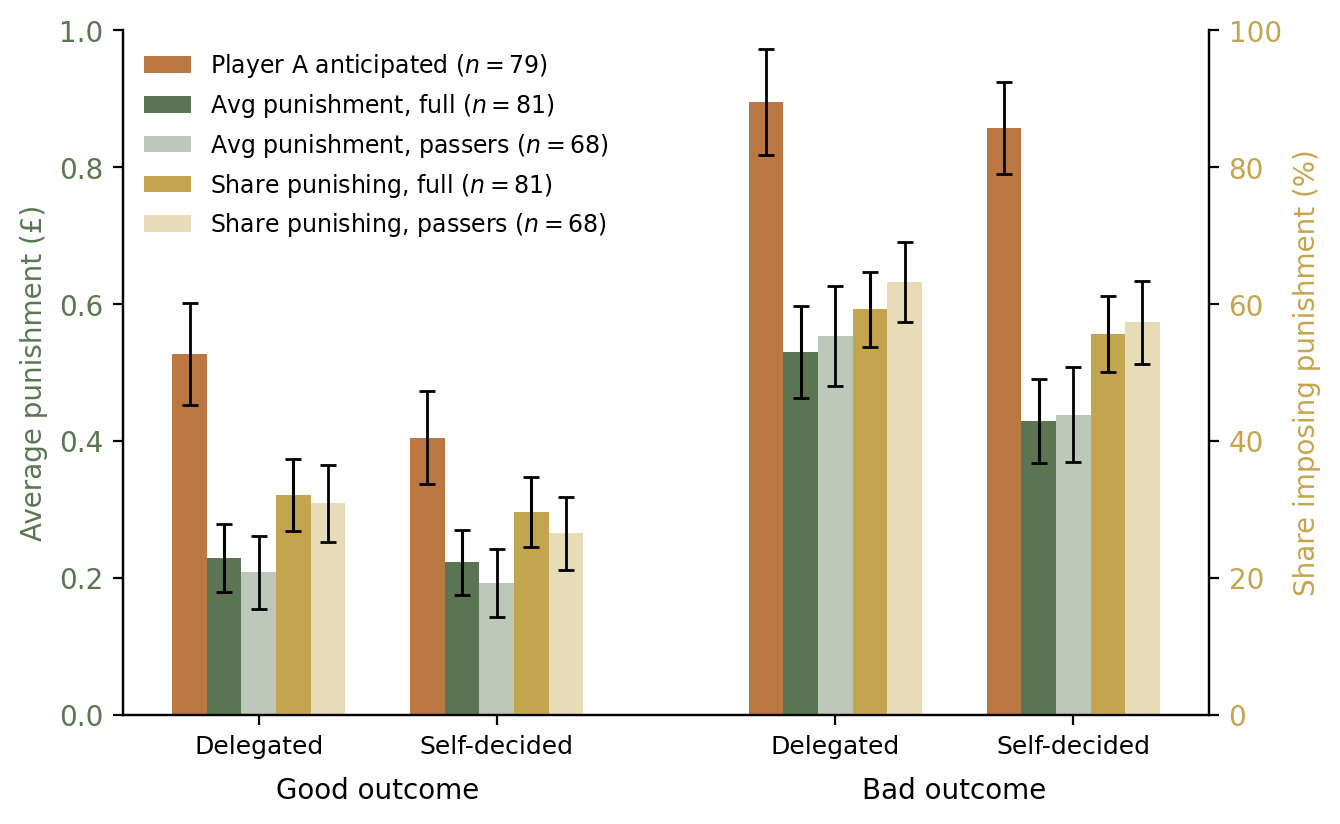
\includegraphics[width=0.65\linewidth]{../quality_reports/exhibits_excl_incredible_guessers/figures/punishment_hypothetical.png}
    \label{fig:excl_punishment_hypothetical}
\end{figure}

\clearpage

%%  from manuscript/main.tex. Every label carries an excl_ prefix, so this
%%  file can coexist with the live exhibits in a single document.
%% =====================================================================

\clearpage
\section*{Exhibits excluding the two incredible weight guessers}

\clearpage
\subsection*{Results}

%% ---------------------------------------------------
%% delegation_shares  [CHANGED]   live location: results.tex:19
%% ---------------------------------------------------
\begin{figure}[!htbp]
    \centering
    \caption{Delegation shares by condition}
    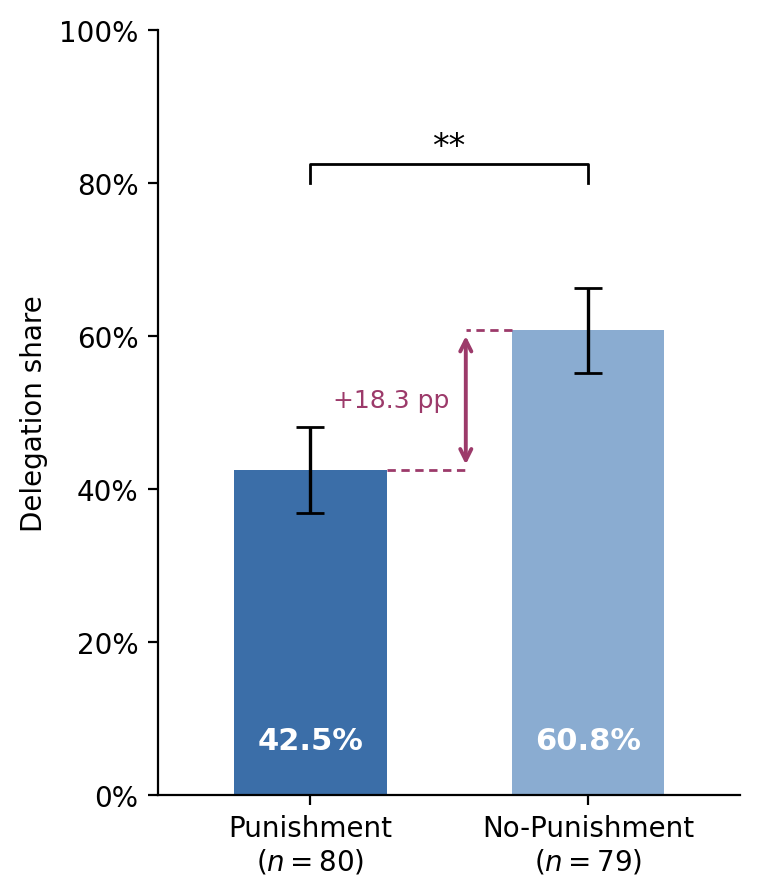
\includegraphics[width=0.5\linewidth]{../quality_reports/exhibits_excl_incredible_guessers/figures/delegation_shares.png}
    \label{fig:excl_delegation_shares}
\end{figure}

\clearpage
%% ---------------------------------------------------
%% reg_delegation  [CHANGED]   live location: results.tex:31
%% ---------------------------------------------------
\begin{table}[!htbp]
\centering
\scriptsize
\caption{Determinants of the delegation decision}
\label{tab:excl_del_decision_determinants}
\begin{tabular}{@{\extracolsep{5pt}}lcccc|c}
\\[-1.8ex]\hline
\hline \\[-1.8ex]
& \multicolumn{5}{c}{Dependent variable: \textit{Delegation}}\\[0.1cm]
& \multicolumn{4}{c}{\textit{Full sample}} & \textit{Passers} \\
\\[-1.8ex] & (1) & (2) & (3) & (4) & (5) \\
\hline \\[-1.8ex]
 Punishment indicator & $-0.462^{**}$ & $-0.473^{**}$ & $-0.537^{**}$ & $-0.489^{**}$ & $-0.589^{**}$ \\
  & $(0.201)$ & $(0.206)$ & $(0.209)$ & $(0.207)$ & $(0.235)$ \\[0.1cm]
 Task performance &  &  & $-0.160^{**}$ &  & $-0.203^{**}$ \\
  &  &  & $(0.081)$ &  & $(0.089)$ \\[0.1cm]
 Perceived performance &  &  &  & $-0.075$ &  \\
  &  &  &  & $(0.057)$ &  \\[0.1cm]
 Age &  & $-0.003$ & $-0.002$ & $-0.002$ & $0.002$ \\
  &  & $(0.009)$ & $(0.009)$ & $(0.009)$ & $(0.011)$ \\[0.1cm]
 Female &  & $0.141$ & $0.194$ & $0.181$ & $0.372$ \\
  &  & $(0.228)$ & $(0.230)$ & $(0.231)$ & $(0.257)$ \\[0.1cm]
 Socio-economic status &  & $-0.044$ & $-0.042$ & $-0.036$ & $-0.086$ \\
  &  & $(0.071)$ & $(0.073)$ & $(0.072)$ & $(0.081)$ \\[0.1cm]
 Went to uni &  & $0.032$ & $0.062$ & $0.020$ & $0.118$ \\
  &  & $(0.228)$ & $(0.226)$ & $(0.227)$ & $(0.248)$ \\[0.1cm]
 Technology score &  & $-0.065$ & $-0.036$ & $-0.056$ & $0.024$ \\
  &  & $(0.093)$ & $(0.096)$ & $(0.093)$ & $(0.109)$ \\[0.1cm]
 Leadership position &  & $0.415^{*}$ & $0.444^{*}$ & $0.411^{*}$ & $0.278$ \\
  &  & $(0.226)$ & $(0.228)$ & $(0.226)$ & $(0.256)$ \\[0.1cm]
 Constant & $0.273^{*}$ & $0.533$ & $0.908$ & $0.801$ & $0.851$ \\
  & $(0.143)$ & $(0.557)$ & $(0.593)$ & $(0.606)$ & $(0.673)$ \\[0.1cm]
\hline \\[-1.8ex]
 AME of Punishment (pp) & $-18.3^{**}$ & $-18.3^{**}$ & $-20.3^{***}$ & $-18.7^{**}$ & $-21.8^{***}$ \\
  & $(p=0.019)$ & $(p=0.019)$ & $(p=0.008)$ & $(p=0.016)$ & $(p=0.009)$ \\
 N & $159$ & $157$ & $157$ & $157$ & $128$ \\
 Pseudo $R^2$ & $0.024$ & $0.042$ & $0.060$ & $0.051$ & $0.077$ \\
\hline
\hline \\[-1.8ex]
\multicolumn{6}{c}{\begin{minipage}{0.85\textwidth}\footnotesize \textit{Note:} Coefficients from a Probit regression of the delegation decision on the Punishment indicator and a set of controls. Robust (HC1) standard errors in parentheses. Significance: $^{*}\,p<0.10$; $^{**}\,p<0.05$; $^{***}\,p<0.01$ (two-sided). Due to missing socio-demographic data, two subjects are dropped in Columns~(2)--(5). The \textit{AME of Punishment} reports the average change in the predicted probability of delegation from introducing the punishment possibility, in percentage points.\end{minipage}}
\end{tabular}
\end{table}

\clearpage

%% ---------------------------------------------------
%% punishment  [IDENTICAL to live]   live location: results.tex:40
%% ---------------------------------------------------
\begin{figure}[!htbp]
    \centering
    \caption{Player~B punishment by delegation and outcome scenario}
    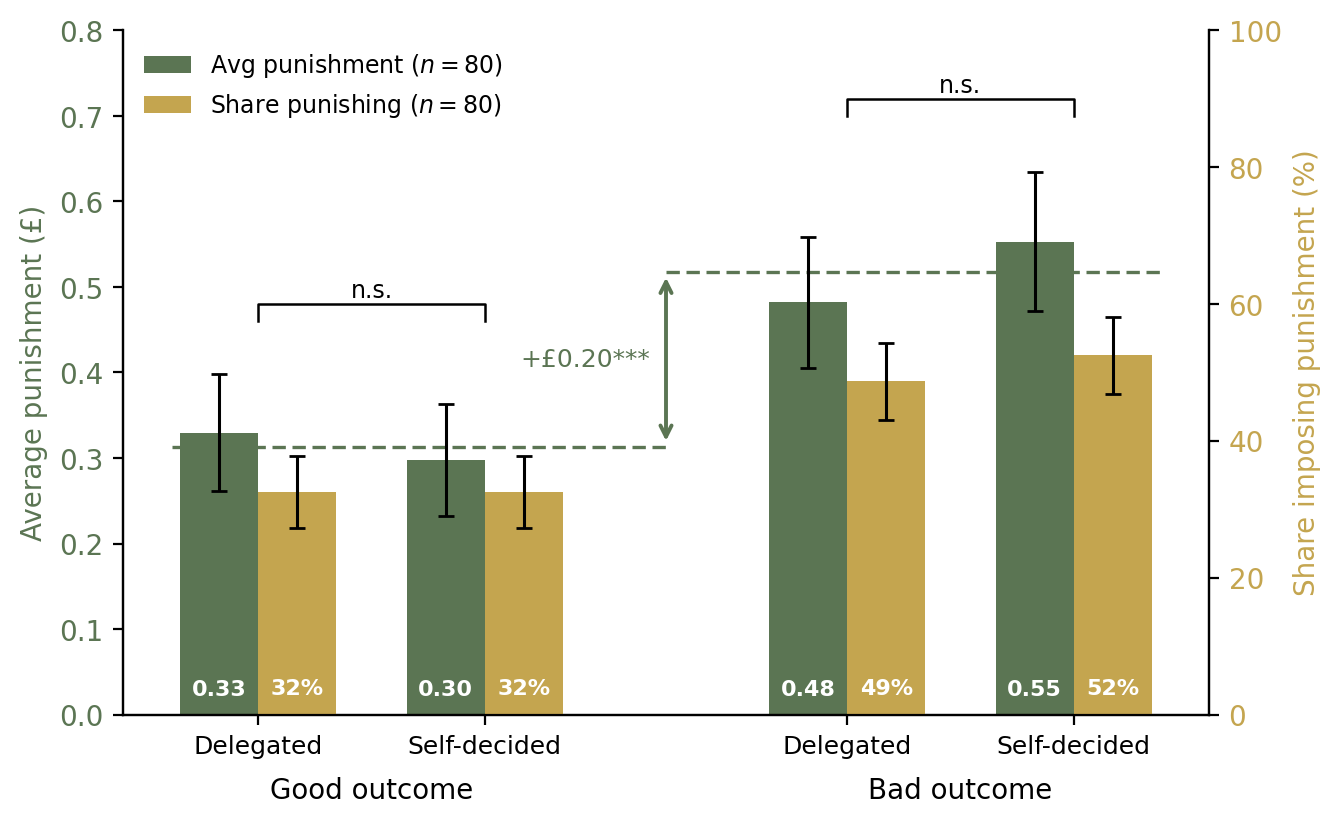
\includegraphics[width=0.75\linewidth]{../quality_reports/exhibits_excl_incredible_guessers/figures/punishment.png}
    \label{fig:excl_punishment}
\end{figure}

\clearpage
%% ---------------------------------------------------
%% reg_punishment  [IDENTICAL to live]   live location: results.tex:58
%% ---------------------------------------------------
\begin{table}[!htbp]
\centering
\scriptsize
\caption{Determinants of Player~B's chosen punishment}
\label{tab:excl_reg_punishment}
\begin{tabular}{@{\extracolsep{5pt}}lcc}
\\[-1.8ex]\hline
\hline \\[-1.8ex]
& \multicolumn{2}{c}{Dependent variable: \textit{Punishment (\pounds)}}\\[0.1cm]
& \textit{Full sample} & \textit{Passers} \\
\\[-1.8ex] & (1) & (2) \\
\hline \\[-1.8ex]
 Delegated & $0.032$ & $0.001$ \\
  & $(0.052)$ & $(0.054)$ \\[0.1cm]
 Bad outcome & $0.256^{***}$ & $0.260^{***}$ \\
  & $(0.071)$ & $(0.080)$ \\[0.1cm]
 Delegated $\times$ Bad outcome & $-0.103^{*}$ & $-0.078$ \\
  & $(0.058)$ & $(0.052)$ \\[0.1cm]
 Player B belief about Player A perf. & $-0.020$ & $0.001$ \\
  & $(0.032)$ & $(0.037)$ \\[0.1cm]
 Age & $0.002$ & $-0.001$ \\
  & $(0.005)$ & $(0.006)$ \\[0.1cm]
 Female & $-0.100$ & $-0.064$ \\
  & $(0.128)$ & $(0.140)$ \\[0.1cm]
 Socio-economic status & $0.083^{*}$ & $0.072$ \\
  & $(0.047)$ & $(0.049)$ \\[0.1cm]
 Went to uni & $-0.196$ & $-0.098$ \\
  & $(0.140)$ & $(0.142)$ \\[0.1cm]
 Technology score & $0.073$ & $0.030$ \\
  & $(0.053)$ & $(0.059)$ \\[0.1cm]
 Leadership position & $0.083$ & $0.061$ \\
  & $(0.142)$ & $(0.164)$ \\[0.1cm]
 Constant & $-0.077$ & $0.020$ \\
  & $(0.328)$ & $(0.374)$ \\[0.1cm]
\hline \\[-1.8ex]
 Observations & $320$ & $268$ \\
 Subjects & $80$ & $67$ \\
 Adj.\ $R^2$ & $0.077$ & $0.030$ \\
\hline
\hline \\[-1.8ex]
\multicolumn{3}{c}{\begin{minipage}{0.75\textwidth}\footnotesize \textit{Note:} OLS regression of Player~B's chosen punishment levels. The sample is stacked over the four (delegation, outcome) scenarios of the strategy method (4 observations per Player~B). Column~(1) uses the full Punishment-condition sample. Column~(2) restricts to Player~Bs who passed the attention check on the punishment-elicitation screen. Standard errors clustered at the Player~B level.\end{minipage}}
\end{tabular}
\end{table}

\clearpage

%% ---------------------------------------------------
%% realized_vs_anticipated  [IDENTICAL to live]   live location: results.tex:86
%% ---------------------------------------------------
\begin{figure}[!htbp]
    \centering
    \caption{Realized vs.\ anticipated punishment, by scenario}
    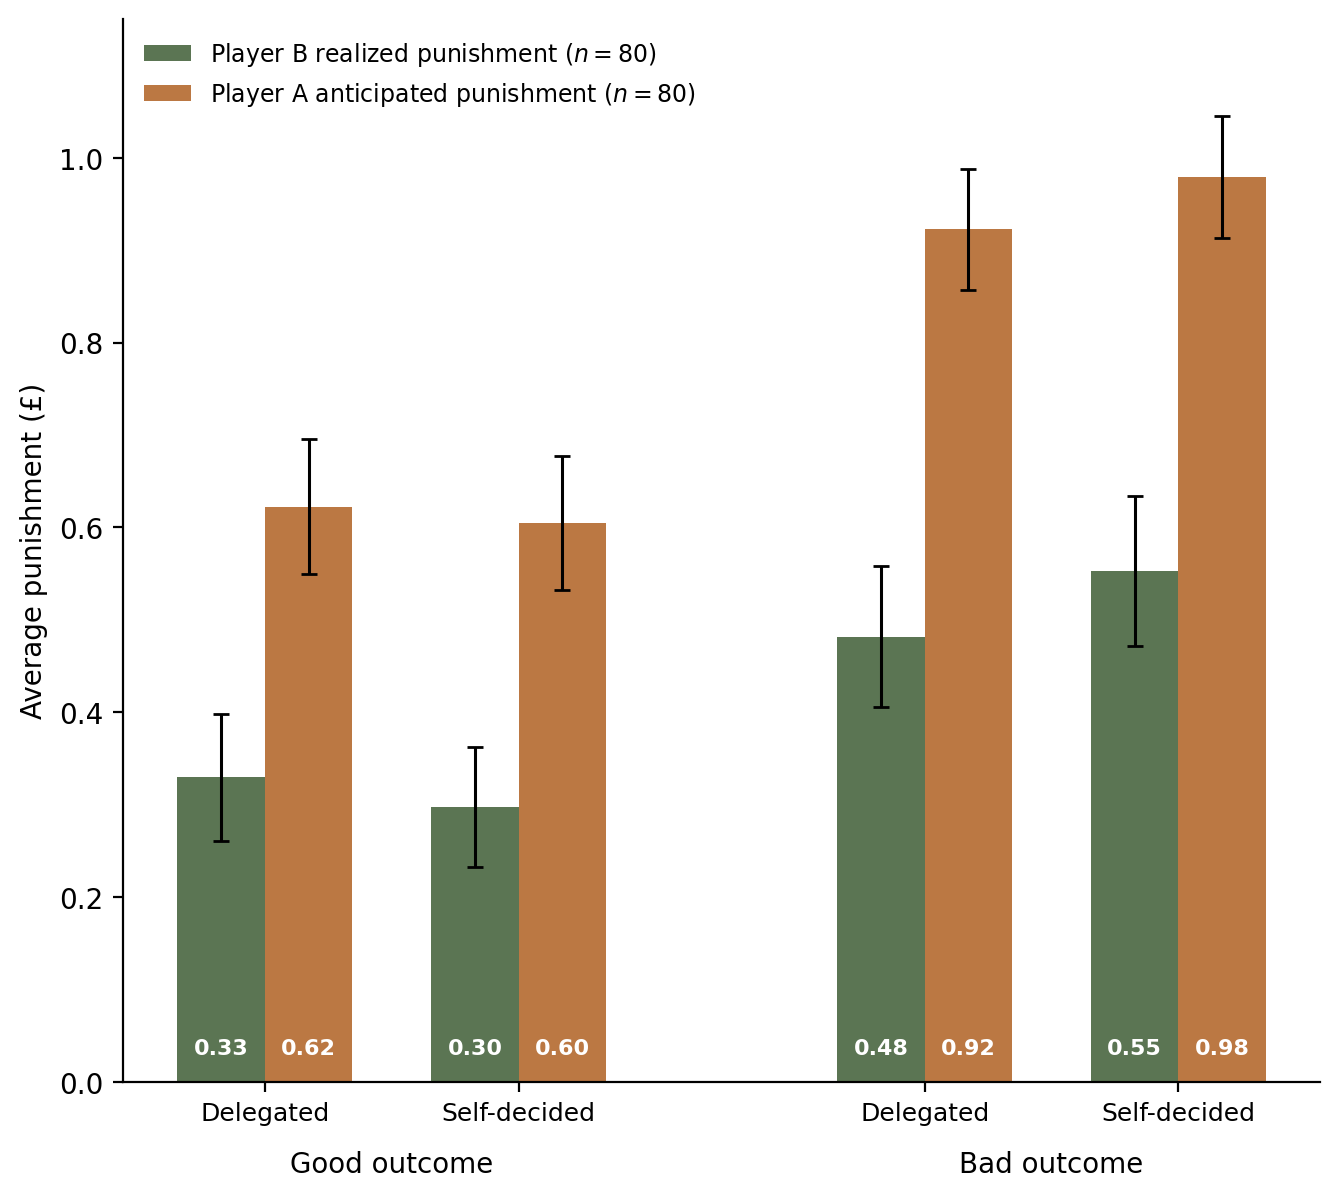
\includegraphics[width=0.75\linewidth]{../quality_reports/exhibits_excl_incredible_guessers/figures/realized_vs_anticipated.png}
    \label{fig:excl_realized_vs_anticipated}
\end{figure}

\clearpage

%% ---------------------------------------------------
%% reg_belief_specs  [IDENTICAL to live]   live location: results.tex:98
%% ---------------------------------------------------
\begin{table}[!htbp]
\centering
\scriptsize
\caption{Delegation and beliefs about punishment}
\label{tab:excl_reg_belief_specs}
\begin{tabular}{@{\extracolsep{5pt}}lcc|ccc}
\\[-1.8ex]\hline
\hline \\[-1.8ex]
& \multicolumn{5}{c}{Dependent variable: \textit{Delegation}}\\[0.1cm]
& \multicolumn{2}{c}{\textit{Full Punishment}} & \multicolumn{3}{c}{\textit{Punishment, passers}} \\
\\[-1.8ex] & (1) & (2) & (3) & (4) & (5) \\
\hline \\[-1.8ex]
 Belief difference, average ($\overline{\Delta}$) & $0.346$ & $0.398$ & $1.661^{**}$ &  &  \\
  & $(0.407)$ & $(0.448)$ & $(0.700)$ &  &  \\[0.1cm]
 Belief difference, weighted by $\Pr(\text{good})$ ($\Delta^{w}$) &  &  &  & $1.992^{**}$ &  \\
  &  &  &  & $(0.794)$ &  \\[0.1cm]
 Belief difference, bad outcome ($\Delta^{\text{bad}}$) &  &  &  &  & $0.590$ \\
  &  &  &  &  & $(0.424)$ \\[0.1cm]
 Belief difference, good outcome ($\Delta^{\text{good}}$) &  &  &  &  & $0.961^{**}$ \\
  &  &  &  &  & $(0.412)$ \\[0.1cm]
 Task performance &  & $-0.208^{*}$ & $-0.362^{***}$ & $-0.342^{**}$ & $-0.381^{***}$ \\
  &  & $(0.111)$ & $(0.136)$ & $(0.142)$ & $(0.138)$ \\[0.1cm]
 Age &  & $0.023^{*}$ & $0.039^{**}$ & $0.040^{**}$ & $0.039^{**}$ \\
  &  & $(0.012)$ & $(0.016)$ & $(0.016)$ & $(0.016)$ \\[0.1cm]
 Female &  & $0.152$ & $0.950^{**}$ & $1.026^{**}$ & $0.845^{*}$ \\
  &  & $(0.350)$ & $(0.427)$ & $(0.406)$ & $(0.444)$ \\[0.1cm]
 Socio-economic status &  & $-0.049$ & $-0.006$ & $-0.055$ & $0.001$ \\
  &  & $(0.111)$ & $(0.131)$ & $(0.133)$ & $(0.126)$ \\[0.1cm]
 Went to uni &  & $0.071$ & $-0.278$ & $-0.169$ & $-0.275$ \\
  &  & $(0.363)$ & $(0.412)$ & $(0.408)$ & $(0.409)$ \\[0.1cm]
 Technology score &  & $-0.061$ & $0.048$ & $0.072$ & $0.033$ \\
  &  & $(0.138)$ & $(0.170)$ & $(0.173)$ & $(0.167)$ \\[0.1cm]
 Leadership position &  & $0.302$ & $-0.301$ & $-0.279$ & $-0.245$ \\
  &  & $(0.312)$ & $(0.408)$ & $(0.408)$ & $(0.411)$ \\[0.1cm]
 Constant & $-0.198$ & $-0.345$ & $-1.228$ & $-1.281$ & $-1.115$ \\
  & $(0.142)$ & $(0.826)$ & $(1.155)$ & $(1.147)$ & $(1.165)$ \\[0.1cm]
\hline \\[-1.8ex]
 AME of belief measure (pp per \pounds 0.10) & $1.3$ & $1.4$ & $4.7^{**}$ & $5.5^{***}$ &  \\
  & $(p=0.388)$ & $(p=0.370)$ & $(p=0.011)$ & $(p=0.006)$ &  \\
 AME: good-outcome difference (pp per \pounds 0.10) &  &  &  &  & $2.7^{**}$ \\
  &  &  &  &  & $(p=0.010)$ \\
 AME: bad-outcome difference (pp per \pounds 0.10) &  &  &  &  & $1.7$ \\
  &  &  &  &  & $(p=0.165)$ \\
 Controls & $\times$ & \checkmark & \checkmark & \checkmark & \checkmark \\
 Passers only & $\times$ & $\times$ & \checkmark & \checkmark & \checkmark \\
 N & $80$ & $78$ & $60$ & $60$ & $60$ \\
 Pseudo $R^2$ & $0.007$ & $0.098$ & $0.248$ & $0.263$ & $0.252$ \\
\hline
\hline \\[-1.8ex]
\multicolumn{6}{c}{\begin{minipage}{0.92\textwidth}\footnotesize \textit{Note:} Probit estimates with robust (HC1) standard errors in parentheses. Sample restricted to the \textit{Punishment} condition throughout. Belief differences are within-subject \textit{(no delegation)}~$-$~\textit{(delegation)} in expected punishment, so positive coefficients indicate that subjects who expect to be punished more harshly for not delegating (relative to delegating) are more likely to delegate. Columns~(1)--(3) use the simple average of the good-outcome and the bad-outcome belief difference. Column~(4) instead weights the good-outcome difference by Player~A's elicited probability of producing the high payoff and the bad-outcome difference by the complementary probability. Column~(5) enters the two differences separately. The \textit{AME} rows report the average marginal effect of the belief measure entered in the respective column on the probability of delegation, in percentage points per \pounds 0.10 increase in the corresponding belief difference.\end{minipage}}
\end{tabular}
\end{table}

\clearpage

%% ---------------------------------------------------
%% performance_overview  [CHANGED]   live location: results.tex:121
%% ---------------------------------------------------
\begin{figure}[!htbp]
    \centering
    \caption{Delegation, performance, and confidence by condition}
    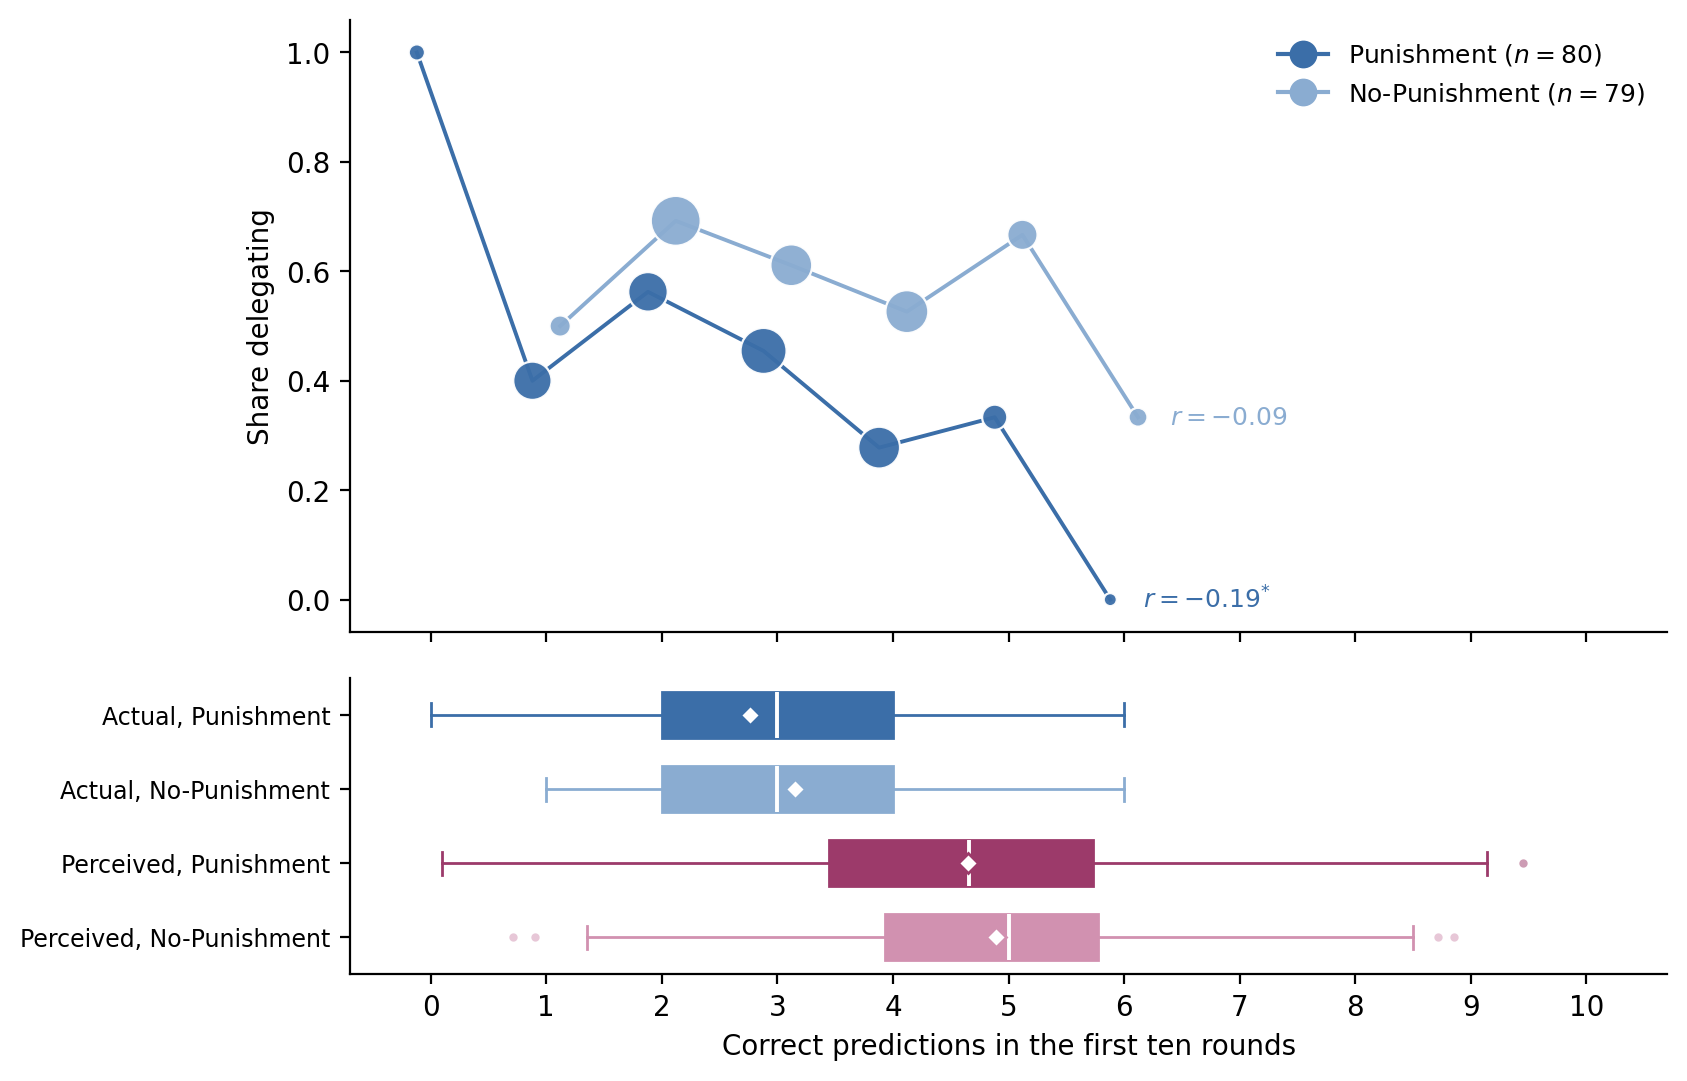
\includegraphics[width=0.9\linewidth]{../quality_reports/exhibits_excl_incredible_guessers/figures/performance_overview.png}
    \label{fig:excl_performance_overview}
\end{figure}

\clearpage

\clearpage
\subsection*{Appendix}

%% ---------------------------------------------------
%% balance_player_a  [CHANGED]   live location: appendix.tex:9
%% ---------------------------------------------------
\begin{table}[!htbp]
    \centering
    \caption{Condition balance --- Player~A}
    \label{tab:excl_treatment_balance}
    \begin{tabular}{l|rrr}
                  Variable &  \textit{Punishment} &  \textit{No-Punishment} &  $p$-value \\ \hline
                           Age &  $39.026$ &  $37.886$ &  $0.557$ \\
                        Female &  $0.487$ &  $0.506$ &  $0.936$ \\
         Socio-economic status &  $5.179$ &  $5.329$ &  $0.542$ \\
                   Went to uni &  $0.575$ &  $0.557$ &  $0.945$ \\
              Technology score &  $2.087$ &  $2.266$ &  $0.366$ \\
           Leadership position &  $0.362$ &  $0.329$ &  $0.783$ \\
    \end{tabular}
    \begin{minipage}{0.95\textwidth}\footnotesize
    \textit{Note:} Mean values by condition for Player~A, with $p$-values from two-sided $t$-tests for continuous variables and Chi-squared tests for binary variables. \textit{Socio-economic status} is self-reported on a $1$--$10$ scale. \textit{Went to uni} indicates a university degree. \textit{Technology score} is constructed from weekly device usage, programming skills, cryptocurrency knowledge, technology use at work, and similar items. \textit{Leadership position} indicates self-reported management or supervisory experience.
    \end{minipage}
\end{table}

\clearpage

%% ---------------------------------------------------
%% reg_punishment_extensive  [IDENTICAL to live]   live location: appendix.tex:19
%% ---------------------------------------------------
\begin{table}[!htbp]
\centering
\scriptsize
\caption{Extensive margin of punishment --- probit for $\Pr(\text{punishment}>0)$}
\label{tab:excl_reg_punishment_extensive}
\begin{tabular}{@{\extracolsep{5pt}}lcc}
\\[-1.8ex]\hline
\hline \\[-1.8ex]
& \multicolumn{2}{c}{Dependent variable: \textit{Any punishment}}\\[0.1cm]
& \textit{Full sample} & \textit{Passers} \\
\\[-1.8ex] & (1) & (2) \\
\hline \\[-1.8ex]
 Delegated & $0.002$ & $-0.042$ \\
  & $(0.077)$ & $(0.078)$ \\[0.1cm]
 Bad outcome & $0.556^{***}$ & $0.563^{***}$ \\
  & $(0.139)$ & $(0.153)$ \\[0.1cm]
 Delegated $\times$ Bad outcome & $-0.099$ & $-0.072$ \\
  & $(0.095)$ & $(0.103)$ \\[0.1cm]
 Player B belief about Player A perf. & $-0.083$ & $-0.030$ \\
  & $(0.075)$ & $(0.082)$ \\[0.1cm]
 Age & $-0.006$ & $-0.013$ \\
  & $(0.013)$ & $(0.015)$ \\[0.1cm]
 Female & $0.115$ & $0.230$ \\
  & $(0.272)$ & $(0.291)$ \\[0.1cm]
 Socio-economic status & $0.160$ & $0.140$ \\
  & $(0.126)$ & $(0.129)$ \\[0.1cm]
 Went to uni & $-0.827^{***}$ & $-0.706^{**}$ \\
  & $(0.320)$ & $(0.349)$ \\[0.1cm]
 Technology score & $0.062$ & $-0.023$ \\
  & $(0.118)$ & $(0.131)$ \\[0.1cm]
 Leadership position & $0.062$ & $-0.071$ \\
  & $(0.293)$ & $(0.321)$ \\[0.1cm]
 Constant & $-0.382$ & $-0.182$ \\
  & $(0.807)$ & $(0.864)$ \\[0.1cm]
\hline \\[-1.8ex]
 AME of Delegated (pp) & $-1.8$ & $-2.9$ \\
  & $(p=0.462)$ & $(p=0.285)$ \\
 AME of Bad outcome (pp) & $18.1^{***}$ & $19.4^{***}$ \\
  & $(p<0.001)$ & $(p<0.001)$ \\
 Observations & $320$ & $268$ \\
 Subjects & $80$ & $67$ \\
 Pseudo $R^2$ & $0.096$ & $0.081$ \\
\hline
\hline \\[-1.8ex]
\multicolumn{3}{c}{\begin{minipage}{0.85\textwidth}\footnotesize \textit{Note:} Probit regression of an indicator for non-zero punishment ($1\{\text{punishment}>0\}$) on a delegation indicator, a bad-outcome indicator, their interaction, Player~B's belief about Player~A's performance, and socio-demographic controls; the sample is stacked over the four (delegation, outcome) cells of the strategy method (4 observations per Player~B). Column~(1) uses the full Punishment-condition sample; Column~(2) restricts to attention-check passers. Standard errors clustered at the Player~B level. The \textit{AME} rows report discrete average marginal effects on the probability of imposing any punishment, in percentage points (for Delegated, the change from $0\to1$ with the interaction moved consistently; for Bad outcome, likewise), computed by counterfactual prediction with p-values from a seeded $400$-replication subject-cluster bootstrap. Significance: $^{*}\,p<0.10$; $^{**}\,p<0.05$; $^{***}\,p<0.01$ (two-sided).\end{minipage}}
\end{tabular}
\end{table}

\clearpage

%% ---------------------------------------------------
%% punishment_passers  [IDENTICAL to live]   live location: appendix.tex:56
%% ---------------------------------------------------
\begin{figure}[!htbp]
    \centering
    \caption{Player~B punishment by delegation and outcome scenario, attention-check passers}
    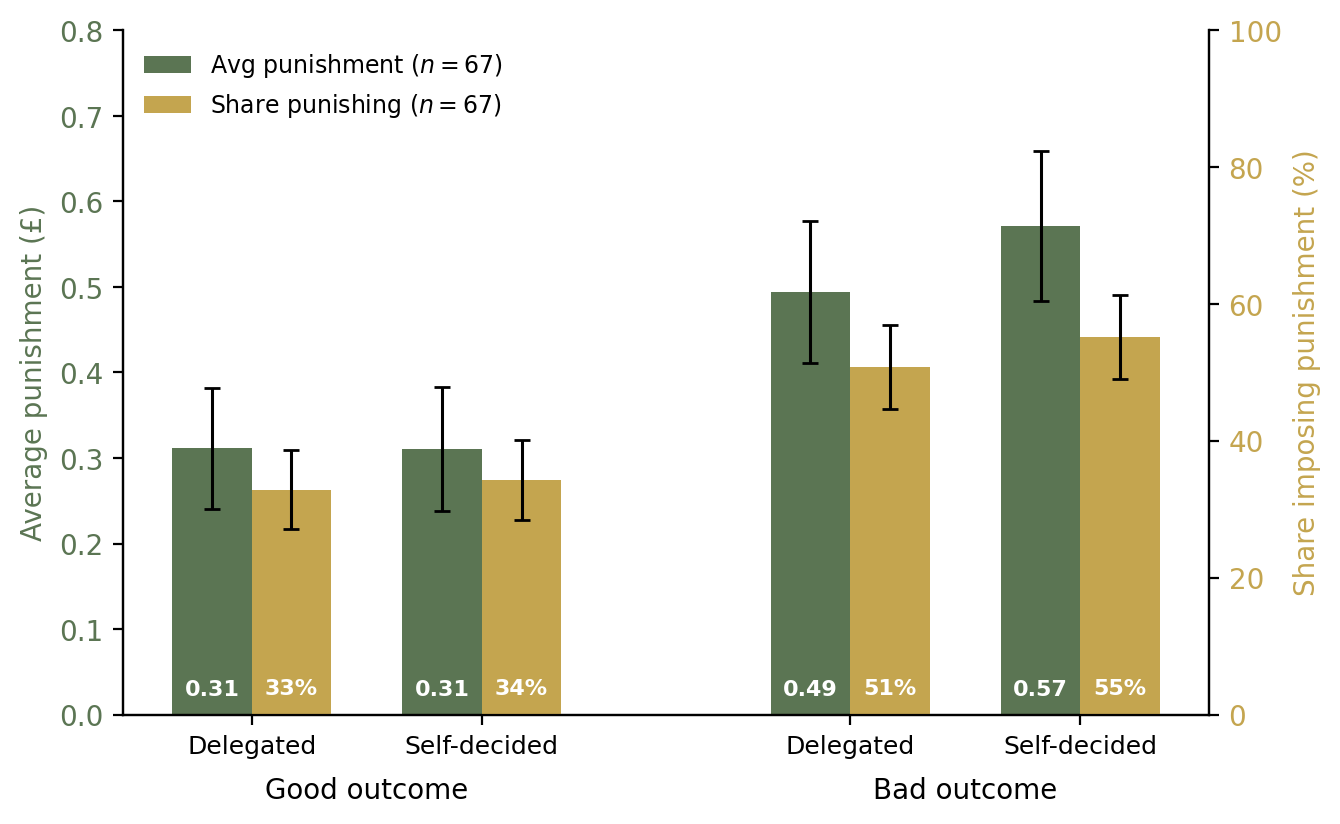
\includegraphics[width=0.65\linewidth]{../quality_reports/exhibits_excl_incredible_guessers/figures/punishment_passers.png}
    \label{fig:excl_punishment_passers}
\end{figure}

\clearpage

%% ---------------------------------------------------
%% realized_vs_anticipated_passers  [IDENTICAL to live]   live location: appendix.tex:67
%% ---------------------------------------------------
\begin{figure}[!htbp]
    \centering
    \caption{Realized vs.\ anticipated punishment, attention-check passers}
    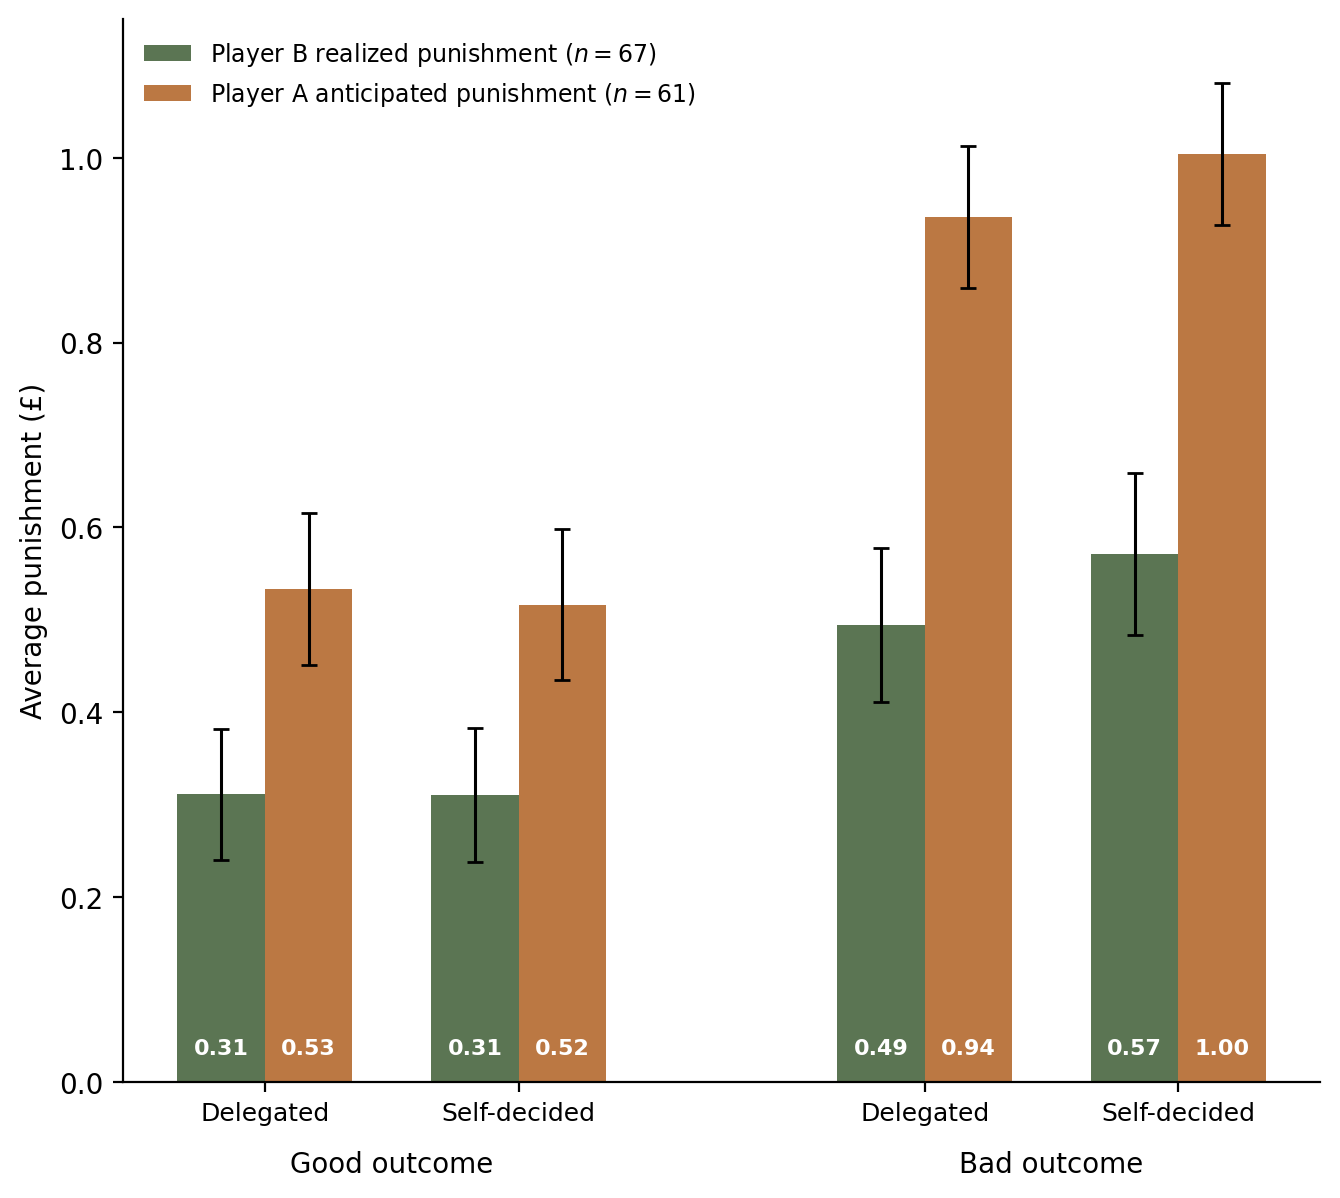
\includegraphics[width=0.75\linewidth]{../quality_reports/exhibits_excl_incredible_guessers/figures/realized_vs_anticipated_passers.png}
    \label{fig:excl_realized_vs_anticipated_passers}
\end{figure}

\clearpage

%% ---------------------------------------------------
%% punishment_hypothetical  [CHANGED]   live location: appendix.tex:83
%% ---------------------------------------------------
\begin{figure}[!htbp]
    \centering
    \caption{Hypothetical punishment by delegation and outcome scenario (\textit{No-Punishment} condition)}
    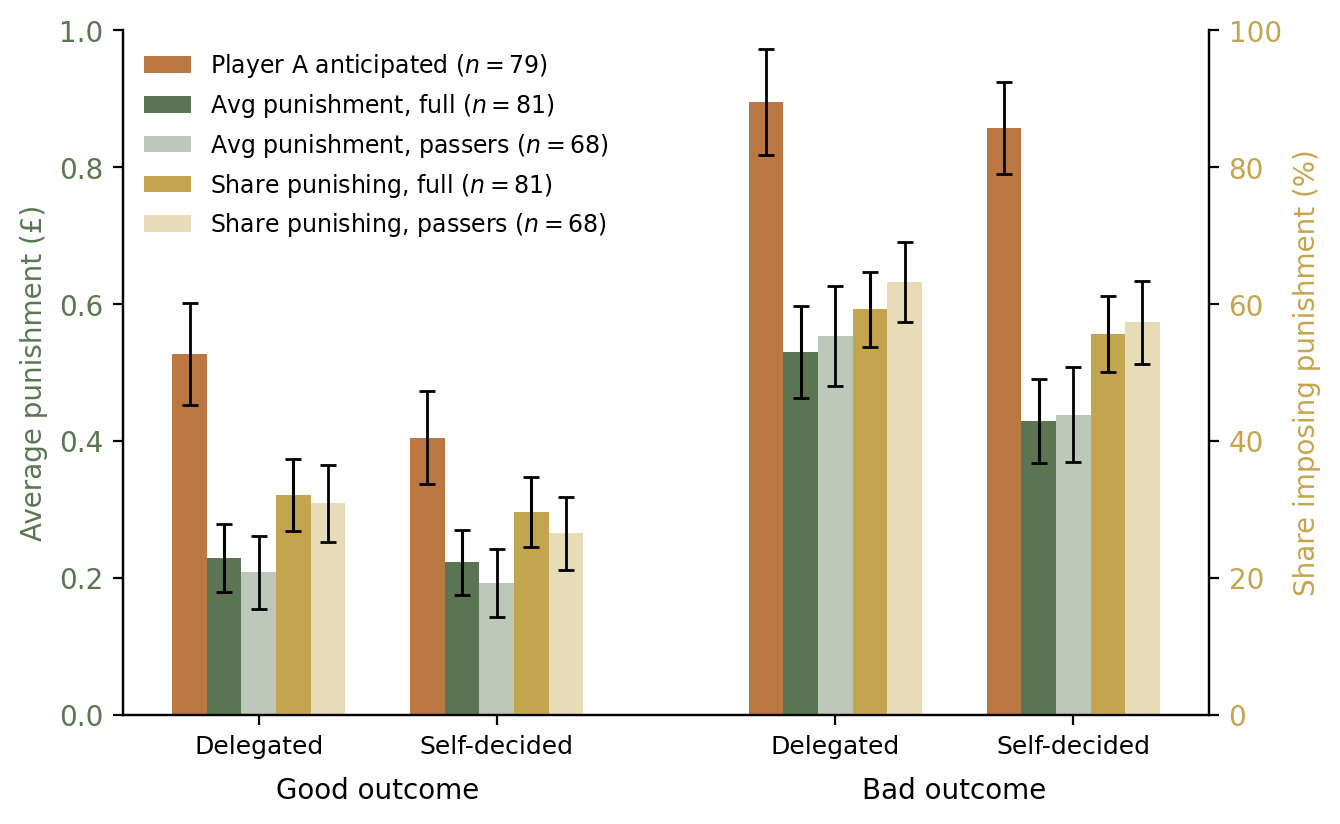
\includegraphics[width=0.65\linewidth]{../quality_reports/exhibits_excl_incredible_guessers/figures/punishment_hypothetical.png}
    \label{fig:excl_punishment_hypothetical}
\end{figure}

\clearpage
